\documentclass{article}
\usepackage{setspace}
%\usepackage{subfigure}

\pagestyle{plain}
\usepackage{amssymb,graphicx,color}
\usepackage{amsfonts}
\usepackage{latexsym}
\usepackage{a4wide}
\usepackage{amsmath}
\usepackage{paper}
\usepackage{mathtools}
\usepackage{algorithm}
\usepackage{algpseudocode}
\usepackage{cfr-lm}
\usepackage{sectsty}
\usepackage{pgf -umlcd}
\usepackage{xcolor}
\usepackage{listings}
\definecolor{light-gray}{gray}{0.95}
\lstdefinestyle{yaml}{
     backgroundcolor=\color{light-gray},
     numbers=left,
     showstringspaces=true,
     basicstyle=\color{black}\scriptsize,
     rulecolor=\color{black},
     string=[s]{'}{'},
     stringstyle=\color{black},
     comment=[l]{:},
     commentstyle=\color{blue},
     morecomment=[l]{-}
 }

% \sectionfont{\fontsize{12}{12}\selectfont}
% \subsectionfont{\fontsize{11}{11}\selectfont}
% \subsectionfont{\fontsize{10}{10}\selectfont}
\newtheorem{theorem}{Theorem}
\newtheorem{lemma}[theorem]{Lemma}
\newtheorem{corollary}[theorem]{Corollary}
\newtheorem{proposition}[theorem]{Proposition}
\newtheorem{remark}[theorem]{Remark}
\newtheorem{definition}[theorem]{Definition}
\newtheorem{fact}[theorem]{Fact}

\newtheorem{problem}[theorem]{Problem}
\newtheorem{exercise}[theorem]{Exercise}
\def \set#1{\{#1\} }
\sectionfont{\fontsize{12}{12}\selectfont}
\subsectionfont{\fontsize{11}{11}\selectfont}
\subsubsectionfont{\fontsize{10}{10}\selectfont}
\def\code#1{\texttt{#1}}
\usepackage[nottoc,notlot,notlof]{tocbibind}
\usepackage{booktabs}
\usepackage{siunitx}

\newenvironment{proof}{
PROOF:
\begin{quotation}}{
$\Box$ \end{quotation}}

\usepackage{xcolor}
\newcommand{\jk}[1]{{\color{blue} [JK: #1]}}
\newcommand{\jw}[1]{{\color{gray} [JW: #1]}}
\newcommand{\vw}[1]{{\color{green} [VW: #1]}}

\newcommand{\calF}{\boldsymbol{\mathcal{F}}}
\newcommand{\bbP}{\mathbb{P}}
\newcommand{\bbR}{\mathbb{R}}
\newcommand{\bbD}{\mathbb{D}}
\newcommand{\bbN}{\mathbb{N}}
\newcommand{\bbE}{\mathbb{E}}
\newcommand{\bbV}{\mathbb{V}}
\newcommand{\bbQ}{\mathbb{Q}}
\newcommand{\bbC}{\mathbb{C}}
\newcommand{\calX}{\mathcal{X}}
\newcommand{\calY}{\mathcal{Y}}
\newcommand{\calZ}{\mathcal{Z}}
\newcommand{\calB}{\mathcal{B}}
\newcommand{\calP}{\mathcal{P}}
\newcommand{\calQ}{\mathcal{Q}}
\newcommand{\calS}{\mathcal{S}}
\newcommand{\calN}{\mathcal{N}}
\newcommand{\calO}{\mathcal{O}}
\newcommand{\calM}{\mathcal{M}}
\newcommand{\KL}{\operatorname{KL}}
\newcommand{\MMD}{\operatorname{MMD}}
\newcommand{\JSD}{\operatorname{JSD}}



\newcommand{\nats}{\mbox{\( \mathbb N \)}}
\newcommand{\rat}{\mbox{\(\mathbb Q\)}}
\newcommand{\rats}{\mbox{\(\mathbb Q\)}}
\newcommand{\reals}{\mbox{\(\mathbb R\)}}
\newcommand{\ints}{\mbox{\(\mathbb Z\)}}
\newcommand{\Cat}{\operatorname{\mathcal{C}}}
\newcommand{\Chol}{\operatorname{Chol}}
\newcommand{\KLD}{\operatorname{\mathbb{KL}}}
\newcommand{\D}{\operatorname{\mathbb{D}}}
\newcommand{\WD}{\operatorname{\mathbb{W}_2}}
\newcommand{\tr}{\operatorname{tr}}
\newcommand{\diag}{\operatorname{diag}}
\newcommand{\GP}{\operatorname{\mathcal{GP}}}
\newcommand{\wc}{\operatorname{{}\cdot{}}}

\DeclareMathOperator*{\argmax}{arg\,max}
\DeclareMathOperator*{\argmin}{arg\,min}
\usepackage{perpage}
\MakePerPage{footnote}
% make sure equation numbers start with the section they are from
\numberwithin{equation}{section}
\counterwithin{table}{section}
%%%%%%%%%%%%%%%%%%%%%%%%%%
\usepackage[
%             left=1.25in,
%             right=1.25in,
            top=1in,
            bottom=1in,
%             % footskip=.25in
            ]{geometry}

\begin{document}

\onehalfspacing
\begin{titlepage}
	\centering
\begin{figure}[h!]
\begin{flushright}
    
\includegraphics[width=.333\textwidth]{thesis_report/figures/ucl_logo.png}
\end{flushright}
\end{figure}
    {}
	\vspace{3cm}

	{\Huge\bfseries Generalised Variational Inference \\ for Gaussian Processes\par}
	% \vfill

	\vspace{1cm}
	{\LARGE James (\textit{Jian Shu}) Wu\par}
	\vspace{0.5cm}
	supervised by\par
    \Large{Veit D. Wild \& Jeremias Knoblauch}\\
	\vfill
	{\large September 2023\par}
 \textsc{MSc Computational Statistics and Machine Learning}\\
	\vspace{1cm}
 \textit{\scriptsize{This report is submitted as part requirement for the MSc Computational Statistics and Machine Learning at University College London. It is substantially the result of my own work except where explicitly indicated in the text. \\ The report may be freely copied and distributed provided the source is explicitly acknowledged.}}

	% \vfill

% Bottom of the page
\end{titlepage}
\pagenumbering{gobble}
\newpage
\setcounter{page}{1}
\pagenumbering{roman}

% This report is submitted as part requirement for the Master's in Computational Statistics \& Machine Learning Degree at University College London (UCL). It is substantially the result of my own work except where explicitly indicated in the text.

% \begin{flushright}
%     \textit{James (Jian Shu) Wu}

%     September 2023
% \end{flushright}
% \newpage

\begin{abstract}
Proposed by \cite{knoblauch2022optimization}, generalised variational inference (GVI) is a learning framework motivated by an optimisation-centric interpretation of Bayesian inference. 
Extending GVI to infinite dimensions, \cite{wild2022generalized} introduces Gaussian Wasserstein inference (GWI) in function spaces. 
GWI demonstrates a new inference approach for variational Gaussian Processes (GPs), circumventing many limitations of previous approaches.
Our work introduces various improvements to GWI for GPs, including new kernel parameterisations such as the NNGP kernels from \cite{novak2019neural}. We also introduce a new learning framework that we call projected GVI (pGVI) for GPs. 
pGVI weakens the GVI assumption of a definite regulariser.
Instead, we propose regularising between scalar projections of the stochastic processes, an approach we call projected regularisation.
We demonstrate that pGVI is a highly flexible and well-performing variational inference framework with significantly cheaper linearly time computational costs compared to the cubic costs of existing approaches.
We also present our learning frameworks through a comprehensive software implementation available on 
\href{https://github.com/jswu18/gvi-gaussian-process}{GitHub}\footnote{For the most up-to-date version, see: \href{https://github.com/jswu18/gvi-gaussian-process}{https://github.com/jswu18/gvi-gaussian-process}}$^{,}$\footnote{
For the last version prior to the submission date, see: \\\href{https://github.com/jswu18/gvi-gaussian-process/tree/a24dd7188f51e06b3e7dca4e2a4847ba05e0f62a}{https://github.com/jswu18/gvi-gaussian-process/tree/a24dd7188f51e06b3e7dca4e2a4847ba05e0f62a}}.
\end{abstract}

\newpage
\section*{Acknowledgements}
\textit{This work would not have been possible without Jeremias Knoblauch and Veit D. Wild. 
Thank you for your guidance and endless patience as I navigated this world of theory while wearing the hardhat of an engineer. 
I look forward to continuing our collaboration into the future.
I’d also like to thank my friends and family who have supported me throughout my life and in particular, this past year. 
}

\hspace*{\fill} \textit{- James}

\newpage
\tableofcontents
\newpage
\pagenumbering{arabic}
\setcounter{page}{1}
\setcounter{section}{-1}
\counterwithin{figure}{section}
% \setcounter{section}{-1}


\newpage
\section{Notation}
We will first make some general remarks regarding the notation used throughout this report. 
We will denote $\mathcal{X}$ as any input space, where $\mathbf{X} \coloneqq \left\{x_n\right\}_{n=1}^N$ is a set of $N$ elements from the input space such that $\mathbf{X} \in \mathcal{X}^N$.
We also indicate $N$ input and response pairs as $\left(\mathbf{X}, \mathbf{Y}\right) \coloneqq \left\{x_n, y_n\right\}_{n=1}^N$, where each input $x_n$ has a corresponding $y_n$ in a response space such as $\mathbb{R}$.
$\boldsymbol{\boldsymbol{\mathcal{F}}}$, $\boldsymbol{\mathcal{Q}}$, and $\boldsymbol{\Gamma}$ will also denote spaces, but will be defined throughout the text as needed.

We will frequently use mappings of the form $m: \mathcal{X} \rightarrow \mathbb{R}$. 
Given $\mathbf{X}$ and $m$, we will construct vectors of the form $\mathbf{m} \in \mathbb{R}^N$ such that each element is
\begin{align}
    \left[\mathbf{m}\right]_{n} \coloneqq m(x_n),
\end{align}
for $n=1,\dots, N$. Whenever we need additional clarity, we will denote $\mathbf{m}$ as $\mathbf{m}_{\mathbf{X}}$ or $m\left(\mathbf{X}\right)$ to indicate its dependence on $\mathbf{X}$ and/or $m$.

We will also use mappings following $k: \mathcal{X} \times \mathcal{X} \rightarrow \mathbb{R}$.
With $\mathbf{X}$ and $k$, we can construct matrices of the form $\mathbf{K} \in \mathbb{R}^{N\times N}$ where
\begin{align}
    \left[\mathbf{K}\right]_{n, n'} \coloneqq k(x_n, x_{n'})
\end{align}
for $n, n'=1,\dots,N$. 
We denote $\mathbf{K}$ as $\mathbf{K}_{\mathbf{X}, \mathbf{X}}$ or $k\left(\mathbf{X}, \mathbf{X}\right)$ whenever necessary.

A Gaussian distribution will be denoted $\mathcal{N}(\cdot, \cdot)$, where 
\begin{align}
    Y \sim \mathcal{N}(\mathbf{m}, \mathbf{K})
\end{align}
with $Y \in \mathbb{R}^N$ indicates that $Y$ is a random vector following a Gaussian distribution having $\mathbf{m} \in \mathbb{R}^N$ as the mean and $\mathbf{K} \in \mathbb{R}^{N \times N}_{\succcurlyeq 0}$ as the covariance. 
The subscript ${\succcurlyeq 0}$ denotes that $\mathbf{K}$ is positive semi-definite.

For any random element $F$, we review the following notation conventions:
\begin{itemize}
    \setlength\itemsep{-0.25em}
    \item sample notation: 
        \begin{align}
            F \sim \mathcal{N}(\cdot, \cdot)
        \end{align}
        as seen previously, which becomes $F \vert \mathbf{Y}$ when $F$ is conditioned on the known element $\mathbf{Y}$,
    \item measure notation: 
        \begin{align}
            \mathbb{P}^F = \mathcal{N}(\cdot, \cdot),
        \end{align}
        where $\mathbb{P}^F$ is the probability measure of $F$ or $\mathbb{P}(F) = \mathcal{N}(\cdot, \cdot)$, becoming $\mathbb{P}(F \vert \mathbf{Y})$ when conditioned, and
    \item probability density notation: 
        \begin{align}
           p(f) = \mathcal{N}(\cdot, \cdot),
        \end{align}
        when there exists a density $p$ with respect to some other measure, most commonly the Lebesgue measure. 
        When conditioned, we denote $p(f\vert \mathbf{Y})$.
\end{itemize}
Sample, measure, and probability density notation will be used interchangeably, whenever appropriate. 
We will also define new notation such as $P \coloneqq \mathbb{P}(F)$ and $Q \coloneqq \mathbb{Q}(F)$, whenever convenient.

Other conventions that we follow include:
\begin{itemize}
    \setlength\itemsep{-0.25em}
    \item $\mathbb{E}_{P}[\wc]$ to denote expectation with respect to $P$,
    \item $\left[\wc\right]^T$ to denote the matrix transpose, and 
    \item $\mathbb{D}[Q, P]$ to denote a divergence between the measures $Q$ and $P$. Other divergences will follow similar notation and will be defined whenever they are used.
\end{itemize}
 

\newpage
\section{Introduction}
Uncertainty quantification is an important research direction within the machine learning community.
As a modelling approach, it can encourage desirable prediction behaviours such as out-of-distribution (OOD) detection. 
In practice, quantifying uncertainty can provide valuable information during high-risk situations and enable better informed decision-making.

% These include Monte-Carlo dropout, an approach based on weight sampling for neural networks, ensemble techniques, quantifying the spread of `disagreement' across a number of different models, and Bayesian approaches, where previous observations are used to quantify our beliefs for new data through the Bayesian posterior.
% This has motivated variational approaches such as \cite{titsias2009variational}.
% However, these approaches have their own limitations with respect to scaleability and restrictive approximation spaces.

There are a number of modelling approaches for uncertainty quantification. 
Bayesian approaches are a common choice and generally provide more theoretically intuitive interpretations of uncertainty compared to other methods. 
Our work focuses on a well-known Bayesian approach called Gaussian processes (GPs), which we review in Section \ref{section:gaussian-processes}.
GPs quantify uncertainty in the function space domain but like most Bayesian approaches, they suffer from mis-specifications and computational intractability. 
The problem of GP intractability has motivated many variational approaches, including the sparse variational GP (svGP) proposed by \cite{titsias2009variational}.
We review the svGP in Section \ref{section:vi-gp}, but by operating within restrictive approximation spaces, we also recognise the limitations of this approach. 
With a review of \cite{knoblauch2022optimization} in Section \ref{section:gvi-for-gps}, we explain how generalised variational inference (GVI) addresses the issues of mis-specification and intractability prevalent in Bayesian inference.
GVI re-contextualises Bayesian modelling within an optimisation-centric learning framework.
This is followed by a review of Gaussian Wasserstein inference (GWI) from \cite{wild2022generalized} later in the same section, which extends GVI to function spaces.
GWI offers a solution to the restrictive approximation spaces of previous variational GP approaches, such as the svGP.

Our contributions begin in Section \ref{section:improving-gwi}, where we present a number of improvements to the GWI learning framework.
This includes new parameterisations for the prior kernel such as the NNGP kernel from \cite{novak2019neural}.
We will also introduce new variational kernels as well as faster numerical approximations of the GWI objective.
This is followed by Section \ref{section:pgvi}, which introduces a new computationally cheap framework we call projected GVI 
(pGVI) for GPs.
pGVI offers more flexibility for defining learning objectives for variational GPs with a new form of regularisation we call projected regularisation.
This computes divergences between scalar projections of GPs.
We also present an experimentation framework for our contributions, summarised in Section \ref{section:experimentation-framework}. 
This includes the development of an extensive software implementation designed for flexibility and scaleability, introducing appropriate abstraction architectures, and following best practices common in the software engineering community. 
This section will also present our experimentation setup, with examples to show it in action. We conclude with Section \ref{section:future-work} proposing future research directions and final thoughts in Section \ref{section:conclusions}.

\newpage
\section{Gaussian Processes}\label{section:gaussian-processes}
Gaussian processes (GPs) are powerful universal function approximators that can be used for both regression and classification tasks. The following sections will review GPs following \cite{rasmussen2003gaussian}, \cite{matthews2017scalable}, and \cite{wild2022generalized}.

\subsection{The Gaussian Process}\label{section:the-gp}
A GP is a stochastic process such that for any $N$ points $\mathbf{X} \coloneqq \left\{ x_n\right\}_{n=1}^N$ where $x_n \in \mathcal{X}$, the corresponding random response vector $Y \in \mathbb{R}^N$ has the Gaussian distribution
\begin{align}
    \label{gp-vector}
    Y \sim \mathcal{N}\left(\mathbf{m}, \mathbf{K}\right),
\end{align}
where $\mathbf{m} \in \mathbb{R}^N$ and $\mathbf{K} \in  \mathbb{R}^{N \times N}_{\succcurlyeq 0}$.
The mean vector $\mathbf{m}$ is constructed through the selection of a mean function mapping $m: \mathcal{X} \rightarrow \mathbb{R}$ such that
\begin{align}
    \label{gp-mean-vector}
    \mathbf{m} \coloneqq \left[ m(x_1) \cdots m(x_N)\right]^T,
\end{align}
while constructing $\mathbf{K}$ involves choosing a kernel function mapping $k: \mathcal{X} \times \mathcal{X} \rightarrow \mathbb{R}$ such that each element of the matrix is the evaluation
\begin{align}
    \label{gp-kernel-matrix}
    \left[\mathbf{K}\right]_{n, n'} \coloneqq k(x_n, x_{n'}),
\end{align}
for $n, n'=1,\dots, N$.
$\mathbf{K}$ is also known as the gram matrix.
Appendix \ref{appendix:positive-definite-kernel} shows that choosing kernel functions defined as inner products of a feature space mapping will ensure that $\mathbf{K}$ is a valid positive semi-definite covariance matrix, as required in (\ref{gp-vector}).


The distribution in (\ref{gp-vector}) is a finite-dimensional instance of the GP random function mapping
\begin{align}
    F \sim \GP(m, k),
    \label{gp}
\end{align}
 where $F \coloneqq \left\{F(x): x \in \mathcal{X}\right\}$ such that a sample path from $F$ has the mapping $f: \mathcal{X} \rightarrow \mathbb{R}$.
In other words, choosing a mean and kernel to construct (\ref{gp}) ensures that \textit{any} finite set of inputs will have a consistent joint Gaussian distribution adhering to (\ref{gp-vector}) such that
\begin{align}
    Y:=\left[F(x_1),\hdots, F(x_N)\right]^T.
\end{align}

GPs are a powerful modelling approach. With minimal restrictions for choosing the mean and kernel function, there are endless possibilities for constructing expressive GP model spaces.
This control and visibility into the model's behaviour is a strong advantage for GPs compared to other approaches.
\cite{novak2019neural} explains that the GP is also an important construct for understanding the theoretical properties of many neural network architectures at initialisation.
Showing that the infinite-width limit of many such architectures can be expressed as a GP has provided a theoretical framework for analysing neural networks, which are typically viewed as black box approaches.
This further motivates the potential and importance of GPs.

\subsection{Gaussian Process Regression}
Consider the regression task where we have $N$ observation pairs $(\mathbf{X}, \mathbf{Y}) \coloneqq \left\{(x_n, y_n)\right\}_{n=1}^{N}$ with inputs $x_n \in \mathcal{X}$ and responses $y_n \in \mathbb{R}$. GP regression models the data generating process as
\begin{align}
    y \sim F(x) + \epsilon,
    \label{regression-data-uncertainties}
\end{align}
where the GP random function mapping $F$ accounts for the epistemic (model) uncertainty and the random scalar $\epsilon$ accounts for the aleatoric (measurement) uncertainty. In this formulation, we assume that the aleatoric uncertainty is homoscedastic of the form
\begin{align}
    \epsilon \sim \mathcal{N} \left(0, \sigma^2\right).
    \label{aleotric-uncertainty}
\end{align}

In GP regression, the Bayesian posterior for a test point $x \in \mathcal{X}$ when conditioned on the training data $\mathbf{X}$ and $\mathbf{Y}$, acts as a `prediction' for the epistemic uncertainty of the test data responses. 
With all terms being Gaussian, this posterior has a closed-form conditional Gaussian expression.
Having also chosen the aleatoric data uncertainty to be modelled as Gaussian in (\ref{aleotric-uncertainty}), GP regression models the test data response $y \in \mathbb{R}$ as
\begin{align}
    y \vert \mathbf{X}, \mathbf{Y}, \sigma^2
    \sim \mathcal{N}\left(\bar{m}(x), \bar{k}(x, x)\right),
    \label{gp-posterior-normal}
\end{align}
with
\begin{align}
    \label{gp-posterior-mean}
    \bar{m}(x) = m(x) + \mathbf{K}_{x, \mathbf{X}} \left(\mathbf{K}_{\mathbf{X}, \mathbf{X}} + \sigma^2 \mathbf{I}\right)^{-1} \left( \mathbf{Y} - \mathbf{m}_{\mathbf{X}}\right)
\end{align}
and
\begin{align}
    \label{gp-posterior-covariance}
    \bar{k}(x, x) = k(x, x) - \mathbf{K}_{x, \mathbf{X}} \left(\mathbf{K}_{\mathbf{X}, \mathbf{X}} + \sigma^2 \mathbf{I}\right)^{-1} \mathbf{K}_{\mathbf{X}, x},
\end{align}
where $\mathbf{m}_{\mathbf{X}}$ is more verbose notation for (\ref{gp-mean-vector}), $\mathbf{K}_{\mathbf{X}, \mathbf{X}}$ is verbose for (\ref{gp-kernel-matrix}), $\mathbf{K}_{x, \mathbf{X}} \in \mathbb{R}^{1 \times N}$ and $\mathbf{K}_{\mathbf{X}, x} \in \mathbb{R}^{N \times 1}$ are gram matrices constructed with $\mathbf{X}$ and $x$ following (\ref{gp-kernel-matrix}), and $\mathbf{I} \in \mathbb{R}^{N \times N}$ is the identity matrix.

\subsection{Gaussian Process Classification}
Consider the classification task where we have $N$ observation pairs $(\mathbf{X}, \mathbf{Y}) \coloneqq \left\{(x_n, y_n)\right\}_{n=1}^{N}$ with inputs $x_n \in \mathcal{X}$ and label responses $y_n \in \{1, \dots, J\}$. In other words, we wish to map each input $x_n$ to one of $J$ labels. Following the approach from \cite{matthews2017scalable}, GPs can be used for classification through the model
\begin{align}
    Y \sim \mathcal{C}\Big(s\left(F_1(x), \dots, F_J(x)\right)\Big),
    \label{gp-classifier}
\end{align}
where we construct $F_j \sim \GP\left(m_j, k_j\right)$ for each label $j=1, \dots J$ such that $F_1, \dots, F_J$ are stochastically independent, and $s: \mathbb{R}^J \rightarrow \Delta(J)$ is a mapping to a $J$ dimensional probability simplex parameterising a categorical distribution $\mathcal{C}$. 
This means that the probability of the $j^{th}$ label is given as
\begin{align}
    \mathbb{P}(Y=j) = s_j(F_1(x), \dots, F_J(x)),
\end{align}
the $j^{th}$ element of the probability simplex from $s$.

\paragraph{The Robust Max Function}\cite{matthews2017scalable} provides a few different choices for $s$ in (\ref{gp-classifier}). We follow \cite{wild2022generalized}, using the robust max function to define the $j^{th}$ element of the probability simplex with
\begin{align}
s_{j}\left(f_1, \dots, f_J\right) = \begin{cases}
      1-\delta, &  \text{if } j = \argmax_{j=1\dots J}\left(f_j\right), \\
      \frac{\delta}{J-1}, & \text{otherwise}, \\
   \end{cases}
   \label{robust-max-function}
\end{align}
where $\delta \in [0, 1]$. 
Typically, $\delta$ is chosen as a very small value (i.e. $1e^{-2}$). 
Constructing the $\Delta(J)$ vector with (\ref{robust-max-function}), we have the probability value of $1-\delta$ for the label of maximum value and $\frac{\delta}{J-1}$ otherwise. 
\cite{wild2022generalized} explains that this formulation provides robustness to outliers, as it only considers the ranking of the GP models for each label.

A benefit of the robust max function is that the expected log-likelihood under the categorical distribution in (\ref{gp-classifier}) becomes analytically tractable. \cite{wild2022generalized} shows that with $N$ input and response pairs, the expected log-likelihood is
\begin{align}
    \mathbb{E} \left[\log p\left(y \vert x\right)\right] \approx \sum_{n=1}^N \log(1-\epsilon) S(x_n, y_n) + \log\left(\frac{\epsilon}{J-1}\right) \left(1-S(x_n, y_n)\right),
    \label{robust-max-function-expected-log-likelihood}
\end{align}
with
\begin{align}
    S(x, j) \coloneqq \frac{1}{\sqrt{\pi}}\sum_{i=1}^{I} w_i \left(\prod_{j'=1, j'\neq j}^J \phi\left(\frac{\xi_i\sqrt{(2 k_{j'}(x, x)}+m_j(x) - m_{j'}(x)}{\sqrt{k_{j'}(x, x)}}\right)\right)
\end{align}
and $\left\{w_i, \xi_i\right\}_{i=1}^I$ being the weights and roots of the Hermite polynomial of order $I \in \mathbb{N}$. $\phi$ is the standard normal cumulative distribution function.

\newpage
\section{Standard Variational Inference for Gaussian Processes}\label{section:vi-gp}
Although they are \textit{analytically} tractable, a major drawback of GP models has been their inability to \textit{computationally} scale with respect to $N$, the number of training points.
Both classification and regression predictive posteriors rely on evaluating the inversion of an $\mathbb{R}^{N \times N}$ matrix in (\ref{gp-posterior-mean}) and (\ref{gp-posterior-covariance}).
This operation has time complexity  $\mathcal{O}(N^3)$ and space complexity $\mathcal{O}(N^2)$, both of which quickly become problematic when scaling to larger-sized training sets.
This problem has been a serious limitation of GPs and has restricted their use to problem domains having smaller-sized data sets.

This section will review standard variational inference (VI) for GPs and in particular, the sparse variational GP (svGP) from \cite{titsias2009variational}, to obtain computationally cheaper approximations of the true predictive posterior.
We will also discuss the challenges of learning within this framework.

\subsection{Standard Variational Inference in Finite Dimensions}\label{section:vi-in-finite-dimensions}
GPs are objects constructed in an infinite dimensional setting, however this section will first review standard VI in a finite dimensional setting.
A Bayesian modelling approach begins by assuming that the data generating process for an observation is conditionally dependent on $M$ unobserved latent random variables $\mathbf{Z} \in \mathcal{X}^M$ through the observation likelihood $p(Y=y\vert \mathbf{Z})$ and the prior $p(\mathbf{Z})$.
These construct a belief update for the generating process called the Bayesian posterior given as
\begin{align}
    p(\mathbf{Z} \vert Y=y) \propto p(Y=y\vert \mathbf{Z})p(\mathbf{Z}),
    \label{bayesian-posterior}
\end{align}
which is often computationally and/or analytically intractable.
This has motivated the need for variational methods like VI to approximate (\ref{bayesian-posterior}).
VI is based on the observation that the Kullback-Leibler (KL) divergence between an arbitrary probability measure $Q \coloneqq \mathbb{Q}(Z)$ and the true Bayesian posterior in (\ref{bayesian-posterior}), which we denote $\mathbb{P}(Z\vert Y)$, can be rewritten as
\begin{align}
    \KLD\left[Q, \mathbb{P}(\mathbf{Z} \vert Y)\right] = L(Q) - \log p(y),
    \label{finite-dimensional-vi-kld}
\end{align}
where $p(y) = \int p(y\vert z)p(z) dz$ is the marginal log-likelihood and
\begin{align}
    L(Q) \coloneqq -\mathbb{E}_{Q}\left[\log p(y \vert \mathbf{Z})\right] + \KLD\left[Q, P\right],
    \label{finite-dimensional-vi-loss}
\end{align}
such that $P \coloneqq \mathbb{P}(Z)$ is the prior and $\KLD\left[\wc, \wc\right]$ denotes the KL divergence.
It follows that
\begin{align}
    \argmin_{Q \in \boldsymbol{Q}} \KLD\left[Q, \mathbb{P}(\mathbf{Z}\vert Y)\right] = \argmin_{Q \in \boldsymbol{Q}} L(Q),
    \label{optimal-approximation-vi}
\end{align}
where $\boldsymbol{Q}$ is a set of candidate probability measures.
In other words, approximating the posterior by minimising (\ref{finite-dimensional-vi-kld}) is equivalent to minimising (\ref{finite-dimensional-vi-loss}). Typically, $\boldsymbol{Q}$ is constructed with respect to a parameter set $\boldsymbol{\Gamma}$ such that
\begin{align}
    \boldsymbol{Q} \coloneqq \left\{Q_{\gamma}: \gamma \in \boldsymbol{\Gamma} \right\},
\end{align}
where $\boldsymbol{\Gamma}$ is a Euclidean parameter space. Therefore solving
\begin{align}
    \gamma^* \in \argmin_{\gamma \in \boldsymbol{\Gamma}} L(Q_{\gamma})
\end{align}
obtains the VI approximation of the Bayesian posterior minimising (\ref{finite-dimensional-vi-kld}), denoted as $Q_{\gamma^*}$. 
Standard VI depends on three important assumptions to ensure a reasonable approximation:
\begin{enumerate}
    \setlength\itemsep{-0.25em}
    \item the parameterised set of measures $\boldsymbol{Q}$ is large enough to contain a reasonable approximation of the true Bayesian posterior,
    \item the parameterisation of $Q$ ensures that $L(Q)$ is tractable or easy to approximate, and
    \item there exists an optimisation procedure that can find a reasonable minimiser $\gamma^*$.
\end{enumerate}
These three assumptions are in tension with each other.
For example, a larger approximation space $\boldsymbol{Q}$ can cause $L(Q)$ to be intractable or create a more difficult optimisation setup.
However in practice, VI can be quite successful if employed by well-informed practitioners of the method.

\subsection[Sparse Variational Gaussian Processes]{Sparse\footnote{Also known as stochastic or scaleable variational Gaussian processes (svGPs)} Variational Gaussian Processes}\label{section:svgp}
To overcome the computationally intractable GP we review \cite{titsias2009variational}, which proposes a variational approximation for the Bayesian predictive posterior in (\ref{gp-posterior-normal}) as
\begin{align}
    \mathbb{Q}(F) \coloneqq \GP(m_Q, r),
\end{align}
where the mean function is
\begin{align}
    \label{svgp-mean}
    m_Q(x) = m_P(x) + \mathbf{K}_{x, \mathbf{Z}}\left(\mathbf{K}_{\mathbf{Z}, \mathbf{Z}}\right)^{-1} \boldsymbol{\mu},
\end{align}
parameterised by $\boldsymbol{\mu} \in \mathbb{R}^M$, and the kernel function is
\begin{align}
r(x, x) = k(x, x) - \mathbf{K}_{x, \mathbf{Z}}\left(\mathbf{K}_{\mathbf{Z}, \mathbf{Z}}\right)^{-1} \mathbf{K}_{\mathbf{Z}, x} + \mathbf{K}_{x, \mathbf{Z}}\left(\mathbf{K}_{\mathbf{Z}, \mathbf{Z}}\right)^{-1}\mathbf{\Sigma}\left(\mathbf{K}_{\mathbf{Z}, \mathbf{Z}}\right)^{-1} \mathbf{K}_{\mathbf{Z}, x}
\label{svgp-covariance}
\end{align}
with $m_P$ and $k$ being the mean and kernel functions of the target GP that we want to approximate, and parameterised by $\mathbf{\Sigma} \in \mathbb{R}^{M\times M}_{\succcurlyeq 0}$.
$\mathbf{Z} \in \mathcal{X}^M$ is $M$ inducing points, typically chosen as some subset of $\mathbf{X}$.
This defines the parameter space
\begin{align}
    \mathbf{\Gamma} = \left\{\boldsymbol{\mu} \in \mathbb{R}^{M}, \mathbf{\Sigma} \in \mathbb{R}^{M\times M}_{\succcurlyeq 0}, \mathbf{Z} \in \mathcal{X}^M \right\}.
    \label{svgp-parameter-space}
\end{align}
Following (\ref{finite-dimensional-vi-loss}), the variational loss for a candidate $Q \coloneqq \mathbb{Q}(F)$ becomes
\begin{align}
L(Q) = \frac{1}{N}\sum_{n-1}^N \mathbb{E}_Q \left[-\log p(y_n \vert F(x_n)\right] + \KLD\left[\mathbb{Q}^F, \mathbb{P}^F\right],
\label{svgp-vi-loss}
\end{align}
where the expectation in (\ref{svgp-vi-loss}) is tractable, since $F(x_n)$ is Gaussian under $Q$.
However it is unclear if the KL divergence between two GPs in the second term is even well-defined and from a practical viewpoint, computable.
\cite{matthews2016sparse} points out that the choice of $m_Q$ and $r$ by \cite{titsias2009variational} ensures that
\begin{align}
    \KLD\left[\GP\left(m_Q, r\right), \GP\left(m_P, k\right)\right] = \KLD\left[\mathcal{N}\left(\boldsymbol{\mu}, \mathbf{\Sigma}\right), \mathcal{N}\left(\mathbf{m}_{\mathbf{Z}}, \mathbf{K}_{\mathbf{Z}, \mathbf{Z}}\right)\right],
\end{align}
reducing the KL divergence between two stochastic processes to
\begin{align}
        \KLD\left[\mathbb{Q}^F, \mathbb{P}^F\right]
    = \frac{1}{2}\left( \tr\left(\left(\mathbf{K}_{\mathbf{Z}, \mathbf{Z}}\right)^{-1} \boldsymbol{\Sigma}\right) - M +
    \left(\mathbf{m}_{\mathbf{Z}} - \boldsymbol{\mu}\right)^T \mathbf{K}_{\mathbf{Z}, \mathbf{Z}}^{-1} \left(\mathbf{m}_{\mathbf{Z}} - \boldsymbol{\mu}\right)+ \log\left(\frac{\det\mathbf{K}_{\mathbf{Z}, \mathbf{Z}}}{\det\boldsymbol{\Sigma}}\right) \right),
    \label{kld-closed-form}
\end{align}
the KL divergence between two finite dimensional Gaussian distributions on $\mathbb{R}^M$.
\cite{titsias2009variational} shows that for a given set of inducing points $\mathbf{Z}$, the optimal choices $\boldsymbol{\mu}^*$ and $\mathbf{\Sigma}^*$ to minimise (\ref{svgp-vi-loss}) have the closed forms
\begin{align}
    \label{svgp-optimal-mean}
    \boldsymbol{\mu}^* = \sigma^{-2}\mathbf{K}_{\mathbf{Z}, \mathbf{Z}} \mathbf{\Psi}^{-1}\mathbf{K}_{\mathbf{Z}, \mathbf{X}}  \left(\mathbf{Y} - \mathbf{m}_\mathbf{X}\right)
\end{align}
and
\begin{align}
    \label{svgp-optimal-covariance}
    \mathbf{\Sigma}^* = \mathbf{K}_{\mathbf{Z}, \mathbf{Z}}  \mathbf{\Psi}^{-1}\mathbf{K}_{\mathbf{Z}, \mathbf{Z}},
\end{align}
where
\begin{align}
    \mathbf{\Psi} \coloneqq \mathbf{K}_{\mathbf{Z}, \mathbf{Z}}  + \sigma^{-2}\mathbf{K}_{\mathbf{Z}, \mathbf{X}} \mathbf{K}_{\mathbf{X}, \mathbf{Z}},
    \label{svgp-optimal-sigma-m}
\end{align}
conveniently eliminating the need for gradient-based optimisations such that $\gamma = \left(\boldsymbol{\mu}^*, \mathbf{\Sigma}^*,  \mathbf{Z}\right)$.

The svGP ensures matrix inversions of $\mathbb{R}^{M \times M}$ matrices with $\mathcal{O}\left(M^3\right)$ time complexity , while the operation $\mathbf{K}_{\mathbf{Z}, \mathbf{X}} \mathbf{K}_{\mathbf{X}, \mathbf{Z}}$ in (\ref{svgp-optimal-sigma-m}) is $\mathcal{O}\left(NM^2\right)$.
Thus, the overall time complexity  of this approach is $\mathcal{O}\left(NM^2\right)$ with space complexity $\mathcal{O}\left(NM\right)$.
This significantly improves the scaleability of GP approaches from the standard GP in Section \ref{section:gaussian-processes}. $M$ is typically chosen as $\mathcal{O}(N^{1/2})$ such that the svGP has $\mathcal{O}(N^{2})$ and $\mathcal{O}(N^{3/2})$ time and space complexity respectively.

This svGP formulation provides a solution to the scaling issues of the GP, but illustrates how the three assumptions of standard VI discussed in Section \ref{section:vi-in-finite-dimensions} can break down.
In particular, the variational set $\mathbf{Q}$ defined by the parameter set $\boldsymbol{\Gamma}$ may not be expressive enough to contain a reasonable approximation of the true Bayesian posterior.
For example, the mean function of the true posterior with a zero mean GP can be expressed as the linear combination
\begin{align}
    \hat{m}(x) = \sum_{n=1}^{N} \alpha_n k(x, x_n) \in \text{span} \left(\left\{k(\cdot, x_1), \dots, k(\cdot, x_N)\right\}\right),
\end{align}
with $\left[\alpha_1 \cdots \alpha_N\right]^T = \mathbf{K}_{\mathbf{X}, \mathbf{X}}^{-1}\mathbf{Y}$.
On the other hand, the corresponding variational mean $m_Q$ in (\ref{svgp-mean}) is only a linear combination within the inducing point space such that
\begin{align}
    m_Q(x) = \sum_{m=1}^{M} \beta_m k(x, z_m) \in \text{span}\left(\left\{k(\cdot, z_1), \dots, k(\cdot, z_M))\right\}\right),
\end{align}
with $\left[\beta_1 \cdots \beta_M\right]^T = \mathbf{K}_{\mathbf{Z}, \mathbf{Z}}^{-1}\boldsymbol{\mu}$.
Choosing $M$ as $\mathcal{O}(N^{1/2})$, it is not unlikely that the inducing point space will be too small to contain a reasonable approximation of $\hat{m}$.
A similar argument can be made for the posterior kernel.
\cite{burt2020understanding} explains that the KL divergence between two GPs is not generally tractable or even finite.
Thus within the Bayesian context of functional VI, we are forced to restrict the variational set $\boldsymbol{Q}$, to obtain a tractable loss $L$.

\subsection{Inducing Point Selection}\label{section:inducing-point-selection}
Within the context of VI, we wish to find an optimal set of inducing points $\mathbf{Z}$ such that
\begin{align}
    \text{span} \left(\left\{k(\cdot, x_1), \dots, k(\cdot, x_N)\right\}\right) \approx \text{span}\left(\left\{k(\cdot, z_1), \dots, k(\cdot, z_M))\right\}\right),
    \label{inducing-point-input-space}
\end{align}
where the inducing points can approximate the majority of the input space. 
Several existing approaches to inducing point selection include \cite{smola2000sparse}, \cite{hensman2015scalable}, \cite{li2016fast}, and \cite{alaoui2015fast}.
Algorithm \ref{alg:inducing-point-selection} reviews an approach from \cite{burt2020convergence}, which proposes an iterative procedure that greedily chooses the next inducing point based on the highest marginal variance in the prior, when conditioned on the currently selected set of inducing points.

\begin{algorithm}
\caption{Greedy Variance Inducing Point Selection}\label{alg:inducing-point-selection}
\begin{algorithmic}
\State $m \leftarrow 1$
 \State $i \leftarrow \argmax \left(\diag\mathbf{K}_{\mathbf{X}, \mathbf{X}}\right) $
 \State $\mathbf{z} \leftarrow \{x_i\}$ \Comment{initialise selection set}
\While{$m < M$}
\State$i \leftarrow \argmax \left(\diag \left(\mathbf{K}_{\mathbf{X}, \mathbf{X}} - \mathbf{K}_{\mathbf{X}, \mathbf{z}} \left(\mathbf{K}_{\mathbf{z}, \mathbf{z}}\right)^{-1}\mathbf{K}_{\mathbf{z}, \mathbf{X}}\right)\right)$
 \State  $\mathbf{z} \leftarrow \mathbf{z} \cup \{x_i\}$ \Comment{add to the current selection set}
 \State  $m \leftarrow m+1$
\EndWhile
\State \Return $\mathbf{z}$
\end{algorithmic}
\end{algorithm}

Figure \ref{fig:inducing-point-algo} compares random selection to Algorithm \ref{alg:inducing-point-selection} with MNIST data, selecting 10 inducing points from 5000 for each digit. 
We see that the greedy variance approach is much more effective at selecting a diverse set of images.
Moreover, the images in Figure \ref{fig:inducing-point-algo} were selected in order from left to right.
The first two images selected by greedy variance are generally two very different variations of the digit.
For example, the first image for `1' is a single line slanted to the right while the second image involves more strokes and slants left, showing how the algorithm greedily minimises the variance across the candidate images.

\begin{figure}[h!]
\small
\centering
\begin{minipage}{.25\textwidth}
  \centering
  \textit{Random Selection}
  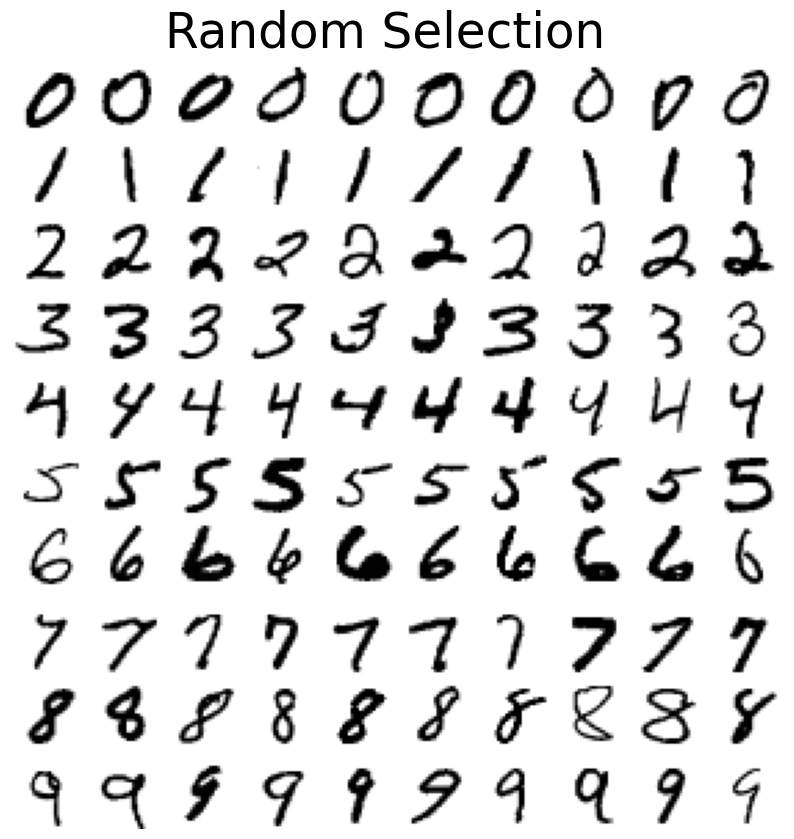
\includegraphics[width=\linewidth, trim={0 0 0 1.5cm},clip]{thesis_report/figures/mnist_inducing_point/random_mnist_inducing_point_selection.png}
\end{minipage}%
\begin{minipage}{.25\textwidth}
  \centering
  \textit{Greedy Variance Selection}
  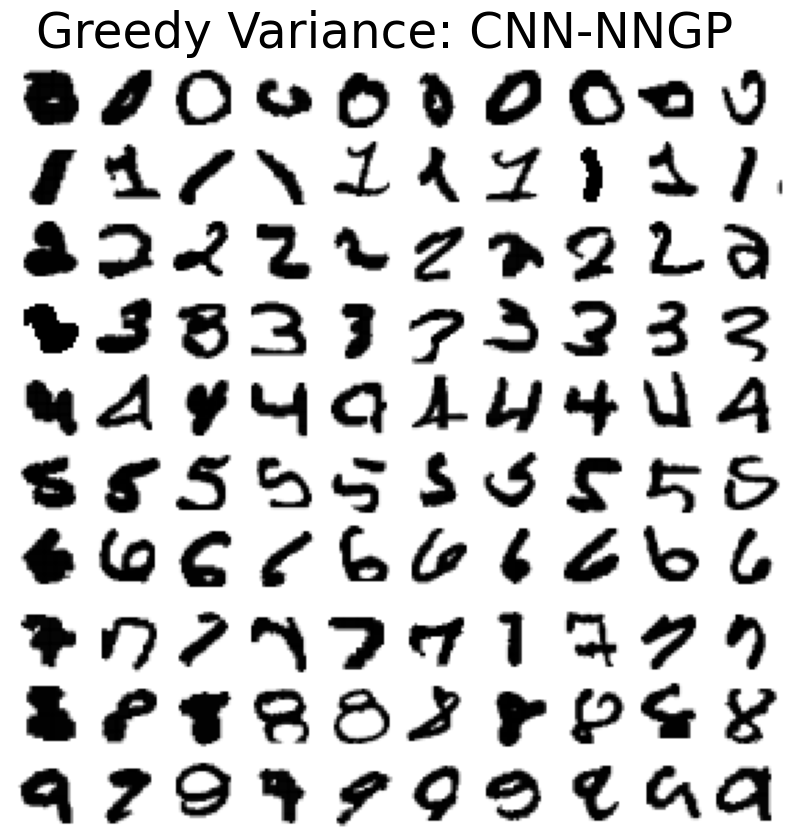
\includegraphics[width=\linewidth, trim={0 0 0 1.5cm},clip]{thesis_report/figures/mnist_inducing_point/greedy_mnist_cnn_nngp_inducing_point_selection.png}
\end{minipage}%
\caption{Random Selection versus Algorithm \ref{alg:inducing-point-selection}}\label{fig:inducing-point-algo}
\end{figure}

\begin{algorithm}[h!]
\caption{Prior Kernel Learning and Inducing Points Selection}\label{alg:inducing-points-prior-gp}
\begin{algorithmic}
\Require $\theta_0$ \Comment{initial hyper-parameters of $k$}
 \State $i \leftarrow 0$
  \State $\mathbf{Z}_0 \leftarrow$ \Call{GreedyVarianceSelection}{$\mathbf{X}$, $\theta_0$} \Comment{via Algorithm \ref{alg:inducing-point-selection} with $k$}
  \State $\mathbf{U}_i \leftarrow \mathbf{Y}\left[\mathbf{X}.\text{index}\left(\mathbf{Z}_0\right)\right]$ \Comment{corresponding inducing point responses}
\While{$\mathbf{Z}_i \neq \mathbf{Z}_{i-1}$}
\State $\theta_{i+1} \leftarrow$ \Call{OptimiseNLL}{$\theta_0$, $\mathbf{Z}_i$, $\mathbf{U}_i$} \Comment{via type-II maximum likelihood on inducing points}
\State $\mathbf{Z}_{i+1} \leftarrow$ \Call{GreedyVarianceSelection}{$\mathbf{X}$, $\theta_{i+1}$}
\State $\mathbf{U}_{i+1} \leftarrow \mathbf{Y}\left[\mathbf{X}.\text{index}\left(\mathbf{Z}_i\right)\right]$
\State $i \leftarrow i+1$
\EndWhile
\State \Return ($\theta_i$, $\mathbf{Z}_i$)
\end{algorithmic}
\end{algorithm}


The inducing point selection method in Algorithm \ref{alg:inducing-point-selection} requires a pre-selected kernel.
However in practice, kernel selection generally involves negative log-likelihood (NLL) optimisation on training data.
In the case of learning the prior GP, this would involve learning the kernel hyper-parameters on the selected inducing points.
This presents a chicken and egg problem.
\cite{burt2020convergence} proposes an EM-like approach, iteratively learning the kernel hyper-parameters and selecting the inducing points with Algorithm \ref{alg:inducing-point-selection} until the convergence of an evidence lower bound.
Our implementation takes a more naive approach, iterating between point selection and NLL minimisation until the inducing points do not change. 
We summarise this approach in Algorithm \ref{alg:inducing-points-prior-gp}.

\begin{figure}[h!]
\small
\centering
\begin{minipage}{.5\textwidth}
  \centering
  \textit{Iteration 1}
  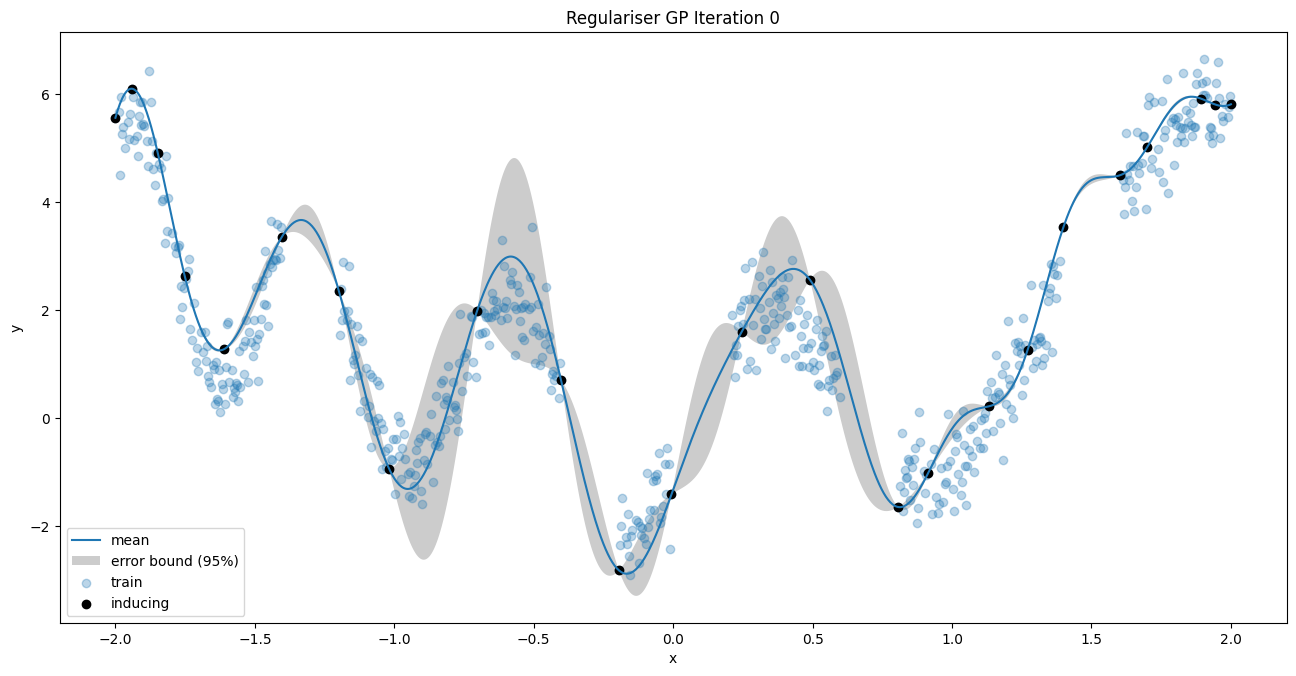
\includegraphics[width=\linewidth, trim={0 0 0 0.77cm},clip]{thesis_report/figures/inducing_points_kernel/iteration-0/prediction.png} 
  \textit{Iteration 3}
  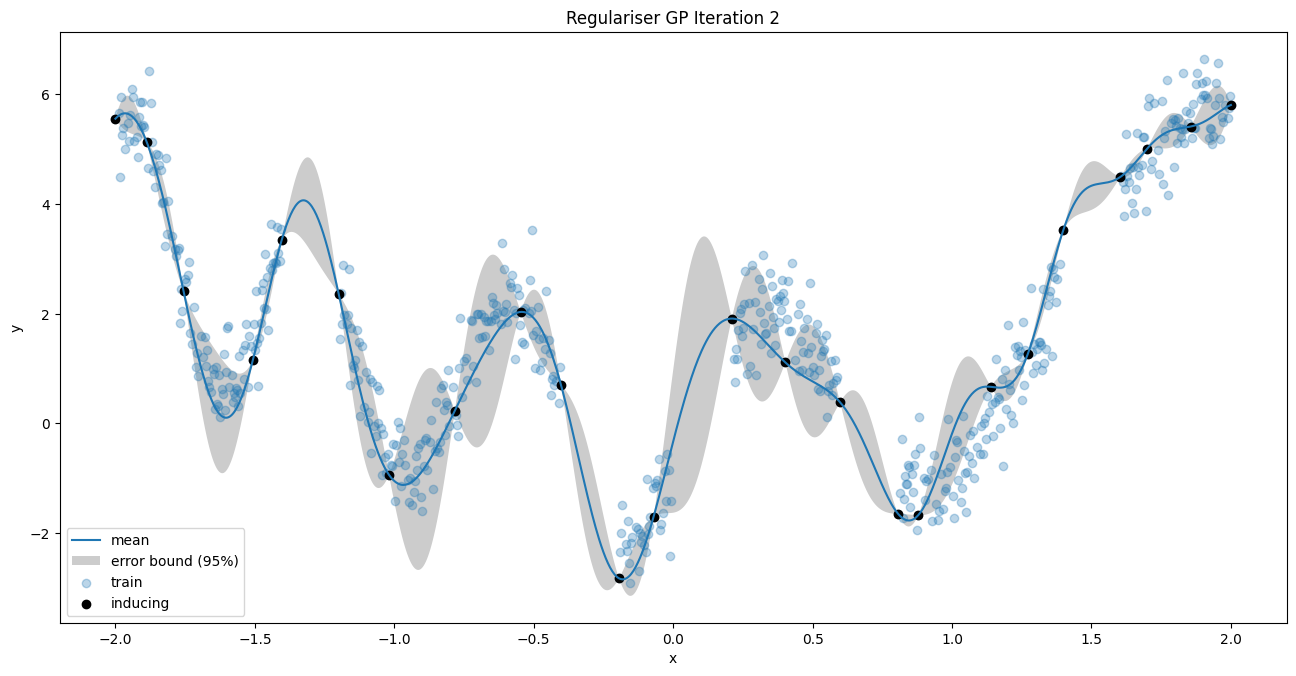
\includegraphics[width=\linewidth, trim={0 0 0 0.77cm},clip]{thesis_report/figures/inducing_points_kernel/iteration-2/prediction.png}
\end{minipage}%
\begin{minipage}{.5\textwidth}
  \centering
  \textit{Iteration 2}
  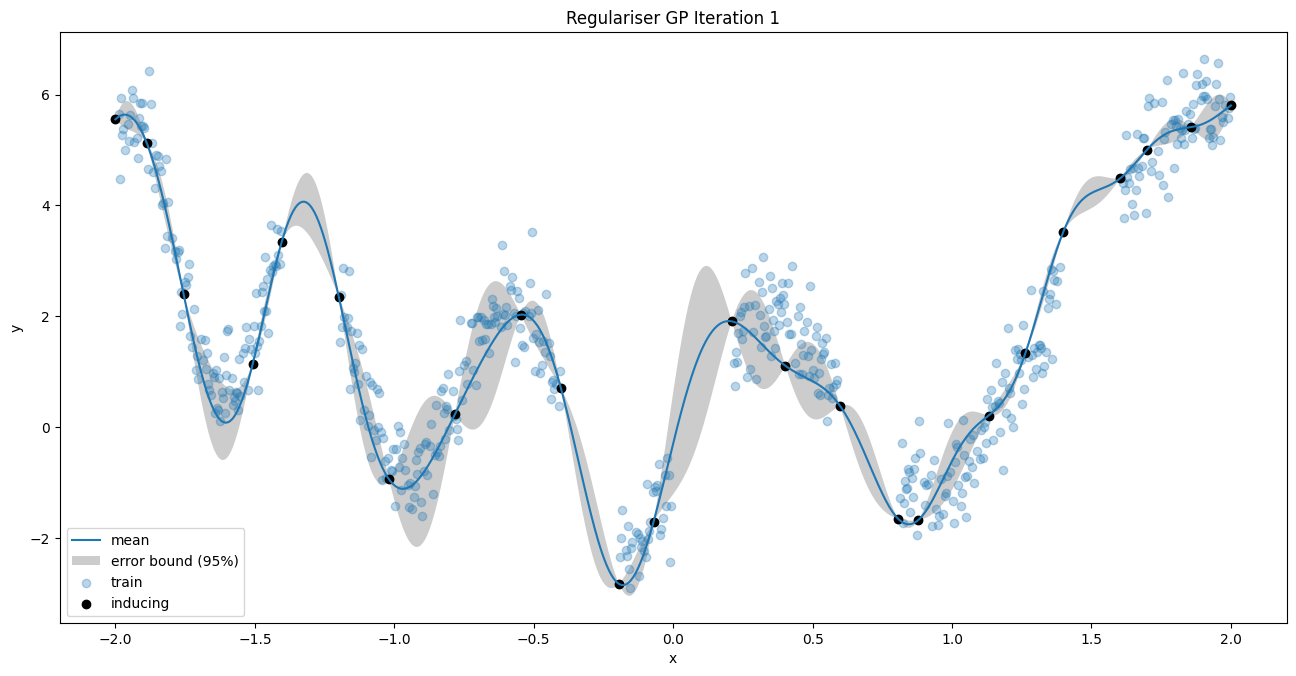
\includegraphics[width=\linewidth, trim={0 0 0 0.77cm},clip]{thesis_report/figures/inducing_points_kernel/iteration-1/prediction.png}
  \textit{Iteration 4}
  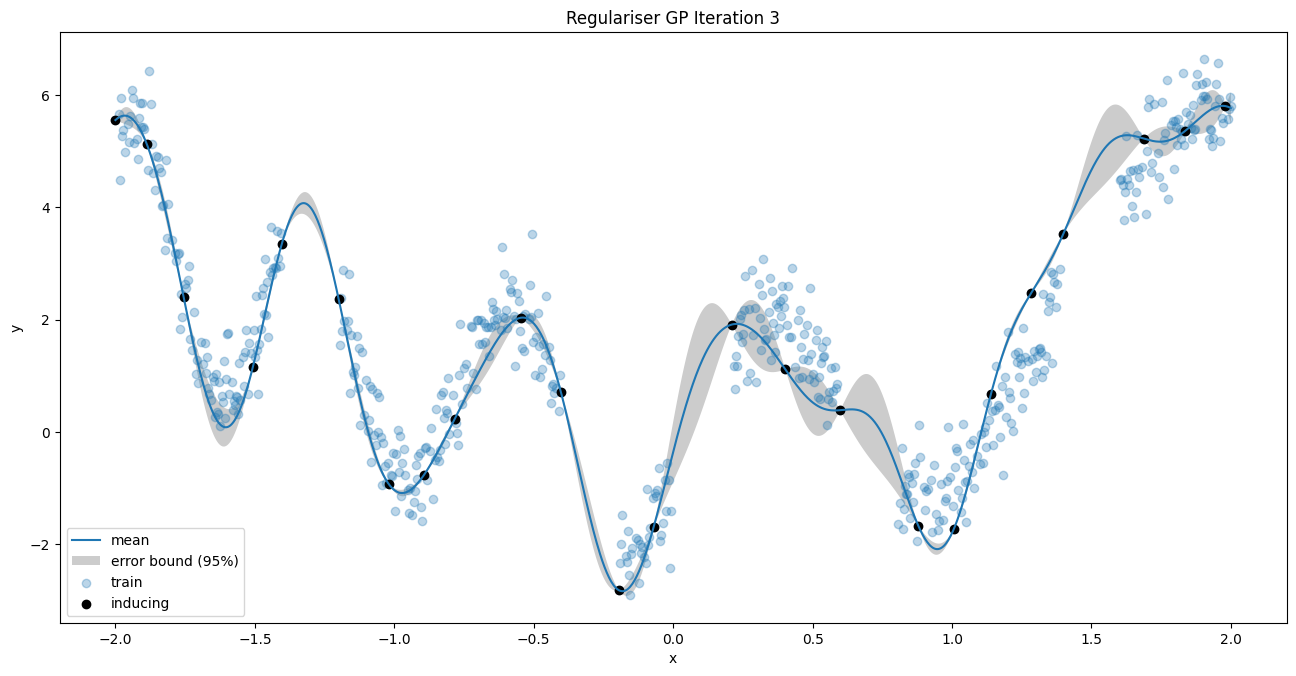
\includegraphics[width=\linewidth, trim={0 0 0 0.77cm},clip]{thesis_report/figures/inducing_points_kernel/iteration-3/prediction.png}
\end{minipage}%
\caption{
Inducing Point Selection for Four Iterations of Algorithm \ref{alg:inducing-points-prior-gp} \textit{(black inducing points and blue training/candidate points)}
}
\label{inducing-points-and-kernel}
\end{figure}

Algorithm \ref{alg:inducing-points-prior-gp} incorporates response data into the inducing point selection process, which did not exist in Algorithm \ref{alg:inducing-point-selection}. 
Learning the kernel with the response data can give more appropriate covariances when comparing candidate points during the inducing points selection of Algorithm \ref{alg:inducing-point-selection}. 
Figure \ref{inducing-points-and-kernel} visualises the inducing points selected in the first four iterations of Algorithm \ref{alg:inducing-points-prior-gp} for a regression problem.
This is overlaid with the Bayesian posterior of a GP parameterised with the learned kernel and zero mean, when conditioned on those selected inducing points. 
This visualises the selection procedure as it attempts to minimise uncertainty over training points, ensuring maximum coverage over the input space.
By learning the kernel in-between iterations, we see that Algorithm \ref{alg:inducing-points-prior-gp} can appropriately adjust the variances on the training data, which would be held fixed during Algorithm \ref{alg:inducing-point-selection}.

In the loop of Algorithm \ref{alg:inducing-point-selection}, each element of the diagonal evaluation has time complexity  $\mathcal{O}(M^2)$ from matrix multiplication, so computing for all $N$ candidate points along the diagonal is $\mathcal{O}(NM^2)$.
The matrix inversion is $\mathcal{O}(M^3)$, but remains a constant when computing each element of the diagonal.
Thus the complexity of selecting each inducing point is $\mathcal{O}(NM^2)$, assuming $M << N$.
Looping to select $M$ inducing points, Algorithm \ref{alg:inducing-point-selection} has $\mathcal{O}(NM^3)$ time complexity .
Choosing $M$ as $\mathcal{O}(N^{1/2})$, we have $\mathcal{O}(N^{5/2})$ time complexity  and $\mathcal{O}(N)$ space complexity. 
Assuming Algorithm \ref{alg:inducing-points-prior-gp} loops for $k$ iterations, we have $\mathcal{O}(k N^{5/2})$ time complexity and the same space complexity as Algorithm \ref{alg:inducing-point-selection}.



\newpage
\section{Generalising Variational Inference for Gaussian Processes}\label{section:gvi-for-gps}
The standard VI objective in (\ref{svgp-vi-loss}) is the root cause of the restrictive variational set for the svGP. 
This is because learning in the standard VI framework necessitates a KL divergence, which is often ill-defined for GPs.

This section will review generalised variational inference (GVI) in finite dimensions from \cite{knoblauch2022optimization}, a framework that does not rely on the KL divergence.
GVI is a fundamental construct for new realisations of variational inference frameworks.
We also review \cite{wild2022generalized}, which extends GVI to an infinite dimensional setting and proposes Gaussian Wasserstein inference (GWI) in function spaces.
GWI constructs a learning framework that avoids the KL divergence for GPs, providing richer approximation spaces for variational learning.

\subsection{Generalised Variational Inference in Finite Dimensions}
Extending the Bayesian posterior from (\ref{bayesian-posterior}) to $N$ observations we have
\begin{align}
    \label{bayesian-posterior-gvi}
    q_B(\mathbf{Z}) \coloneqq p(\mathbf{Z}\vert Y=y) \propto p(\mathbf{Z}) \prod_{n=1}^N p(Y=y_n \vert \mathbf{Z}),
\end{align}
where $p(\mathbf{Z})$ is the prior for the latent variables and $p(Y=y \vert \mathbf{Z})$ is the likelihood of an observation.
The Bayesian posterior $q_B(\mathbf{Z})$ is traditionally viewed as an updated belief for the latent variables by incorporating the likelihood evaluation of new observations.
This interpretation is commonly cited in the context of statistical modelling, where practitioners are focused on obtaining the model specification that characterises an underlying data generating process. 
The validity of this belief update relies on three assumptions:
\begin{enumerate}
    \setlength\itemsep{-0.25em}
    \item a well-specified prior,
    \item a well-specified likelihood, and
    \item an analytically and/or computationally tractable posterior, or the existence of a tractable and reasonable VI approximation,
\end{enumerate}
which are often violated in settings of larger-scaled models like Bayesian Neural Networks (BNNs).

In BNNs, Gaussian priors are generally chosen for computational convenience and are most likely mis-specified in the Bayesian context.
The likelihood evaluation of BNNs are also most definitely mis-specified, as it's unlikely that evaluating such an over-parameterised model would provide any meaningful insights into the data likelihood.
Finally, the posterior of BNNs are often approximated either through samplers or variational approximations.
To achieve sampling convergence, larger-scaled models may require much more computational resources and time than is practically available.
Moreover a reasonable variational approximation is also not always guaranteed, as discussed in Section \ref{section:vi-in-finite-dimensions}.

\cite{knoblauch2022optimization} introduces a new interpretation of the Bayesian posterior, showing that it solves the optimisation problem
\begin{align}
    q_B(Z) = \argmin_{Q \in \boldsymbol{Q}} \left\{\mathbb{E}_{Q}\left[\sum_{n=1}^N \ell \left(\mathbf{Z}, y_n\right)\right] + \mathbb{D}\left[Q, P\right]\right\}
    \label{gvi-posterior}
\end{align}
when choosing $\boldsymbol{Q}$ as the space of all probability measures on $\mathbf{Z}$, the negative log-likelihood $\ell(\mathbf{Z}, y) =-\log p\left(y \vert \mathbf{Z}\right)$,  and the KL divergence $\mathbb{D}\left[Q, P\right] = \KLD\left[Q, P\right]$ with $P$ as the prior.
More generally, $\ell$ is called the loss function and $\mathbb{D}$ is the divergence. With this interpretation, the Bayesian posterior is the solution of a regularised empirical risk minimisation problem.

Framed through optimisation, the Bayesian posterior will always be a valid solution of (\ref{gvi-posterior}), regardless of the three assumptions required to ensure a valid Bayesian belief update.
This is more in-tune with practitioners of larger-scaled models who focus on obtaining superior predictive performance rather than correct model specification.
\cite{knoblauch2022optimization} also shows that by generalising the Bayesian posterior within the learning framework of (\ref{gvi-posterior}), any choice of prior $P$, valid divergence $\mathbb{D}$, loss $\ell$, and approximation set $\boldsymbol{Q}$ will result in a generalised posterior that maintains interpretations as a belief update.
This more flexible inference approach will motivate the replacement of the KL divergence between GPs that was problematic in standard VI.

\subsection{Generalised Variational Inference on Function Spaces}
This section reviews \cite{wild2022generalized}, which extends GVI to infinite dimensional settings to quantify uncertainties on function spaces and proposes  a new framework for variational learning of GPs.
\cite{wild2022generalized} shows that GVI in function spaces involves solving
\begin{align}
    Q^* = \argmin_{Q \in \boldsymbol{Q}} \left\{\mathbb{E}_{Q}\left[\sum_{n=1}^{N}\ell(F, y_n)\right] + \mathbb{D}\left[Q, \mathbb{P}(F)\right]\right\},
    \label{gvi-posterior-in-fs}
\end{align}
where $Q \in \boldsymbol{Q}$ is a variational family of probability measures on a function space $\boldsymbol{\mathcal{F}}$ and $\mathbb{P}(F)$ is a prior on $\boldsymbol{\mathcal{F}}$.
\cite{wild2022generalized} explains that the Kolmogorov Extension Theorem guarantees that for every GP, there exists a corresponding Gaussian measure (GM). 
This GM is usually over the trivial function space $\boldsymbol{\mathcal{F}} = \left\{f: \mathcal{X} \rightarrow \mathbb{R}\right\}$.
However, this space is highly prone to support mis-match and ensuring a tractable KL on $\boldsymbol{\mathcal{F}}$ requires heavy restrictions on the variational family $\boldsymbol{Q}$, as discussed in Section \ref{section:svgp}.
Instead, \cite{wild2022generalized} identifies the existence of GPs with corresponding GMs on the Hilbert space of square integrable functions $\mathcal{L}^2\left(\mathcal{X}, \rho, \mathbb{R}\right)$ when the mean satisfies
\begin{align}
    m \in \mathcal{L}^2\left(\mathcal{X}, \rho, \mathbb{R}\right)
    \label{l2-mean}
\end{align}
and the kernel satisfies
\begin{align}
    \int k(x, x) d\rho(x) < \infty,
    \label{l2-kernel}
\end{align}
also known as the trace-class kernel condition.
These conditions guarantee that sample functions from the GP will have square-integrable paths such that there exists $\mathbb{P} \coloneqq \mathcal{N}(m, C)$, a GM on $\mathcal{L}^2$ with the same mean $m$ and a covariance operator
\begin{align}
    C(f) \coloneqq \int_{\mathcal{X}} k(\cdot, x) f(x) d\rho(x),
\end{align}
for any function $f \in \mathcal{L}^2$.
With the GVI objective in (\ref{gvi-posterior-in-fs}), \cite{wild2022generalized} proposes Gaussian Wasserstein inference (GWI), which replaces the KL divergence from standard VI with the squared 2-Wasserstein distance between GMs on Hilbert spaces 
\begin{align}
    \mathbb{W}\left[Q, P\right]^2 = \left\|m_P - m_Q\right\|_2^2 + \tr\left(C_P\right) + \tr\left(C_Q\right) - 2 \tr \left[\left(\left(C_P\right)^{1/2} C_Q \left(C_P\right)^{1/2} \right)^{1/2}\right],
    \label{wasserstein-distance}
\end{align}
which is always well-defined and does not have the support mis-match problem of the KL divergence.
The subscripts denote the respective GM of each term, $\tr$ is the trace of an operator, and $(C)^{1/2}$ denotes the square root of the positive self-adjoint operator $C$.
Most mean functions satisfy (\ref{l2-mean}) and most kernels satisfy (\ref{l2-kernel}), ensuring the existence of the corresponding Gaussian measures $P$ and $Q$ on $\mathcal{L}^2$.
This provides significantly more freedom for the variational set $\boldsymbol{Q}$ than the svGP approach from \cite{titsias2009variational}.

With GWI, \cite{wild2022generalized} proposes GWI-net, a variational GP parameterised with a neural network mean to replace the svGP mean in (\ref{svgp-mean}).
The experimental results of this approach in \cite{wild2022generalized} show promising potential in both regression and classification tasks.

\newpage

\section{Improving Gaussian Wasserstein Inference}\label{section:improving-gwi}
In this section, we propose improvements to GWI for GPs, the function space GVI framework from \cite{wild2022generalized}.
We introduce new prior and variational kernels for GWI, further exploring the flexibility of the learning framework.
We also introduce a new modular GWI learning procedure.
GPs learned with this procedure will be called GWI-GPs.
Finally, we introduce numerical approximations of the Wasserstein distance that significantly improves inference speed.

\subsection{Improved Kernel Selection}
The GWI framework is parameterised in terms of the infinite-dimensional parameters:
\begin{itemize}
    \setlength\itemsep{-0.25em}
    \item $m_P \in \mathcal{L}^2$, a prior mean function,
    \item $k: \mathcal{X} \times \mathcal{X} \rightarrow \mathbb{R}$, a prior (trace-class) kernel,
    \item $m_Q \in \mathcal{L}^2$, a variational mean function, and
    \item $r: \mathcal{X} \times \mathcal{X} \rightarrow \mathbb{R}$, a variational (trace-class) kernel
\end{itemize}
to construct the objective in (\ref{gvi-posterior-in-fs}). \cite{wild2022generalized} proposes GWI-net, parameterising $m_P$ as the zero mean function, $k$ as the ARD kernel, $m_Q$ as a neural network, and $r$ as the svGP kernel.
The following sections will introduce new parameterisations for the prior and variational kernels.

\subsubsection{Prior Kernels}\label{prior-kernels}
The GWI-net construction from \cite{wild2022generalized} uses an ARD kernel for the prior given as
\begin{align}
    k(x, x') = \sigma^2_f \exp\left(-\frac{1}{2} \sum_{d=1}^D \frac{1}{\alpha_d^2}(x_d-x_d')^2\right),
\end{align}
where $\sigma_f > 0$ is the kernel scaling factor and for each dimension $d=1, \dots, D$, $\alpha_d >0$ is the corresponding length-scale.
In structured data settings like images when it is important to learn correlations between features, having an independent length-scale for each dimension can be less effective.
We propose using kernels that are better suited for structured data settings. These include the neural network Gaussian process kernels (NNGP kernels) from \cite{novak2019neural} and a form of neural network kernels that we will call custom feature mapping kernels.

\paragraph{NNGP Kernels} \cite{novak2019neural} shows that NNGP kernels are the infinite-width limit of neural network architectures at initialisation.
We suggest choosing NNGP kernels with architectures known to be suitable for the given data domain (i.e. a convolutional neural network (CNN) for image data).
The learnable hyper-parameters of NNGP kernels are the variances of the weights and biases for each infinite-width limit layer.

Figure \ref{fig:mnist-inducing-points} compares inducing point selection of different kernels for MNIST data (FCNN denotes a fully connected neural network). 
Using Algorithm \ref{alg:inducing-point-selection}, we selected 10 images from 5000 for each digit.
We also included random selection as a control for visual comparison.
We observed that NNGP kernels are much better at selecting different instances of the same digit, providing better coverage of the data variation.
On the other hand, the ARD kernel is comparable to random selection. 
This motivates the use of NNGP kernels in more structured data settings.
These experiments were performed without any training on the kernel hyper-parameters.
\begin{figure}[h!]
\small
\centering
\begin{minipage}{.25\textwidth}
  \centering
  \textit{Random Selection}
  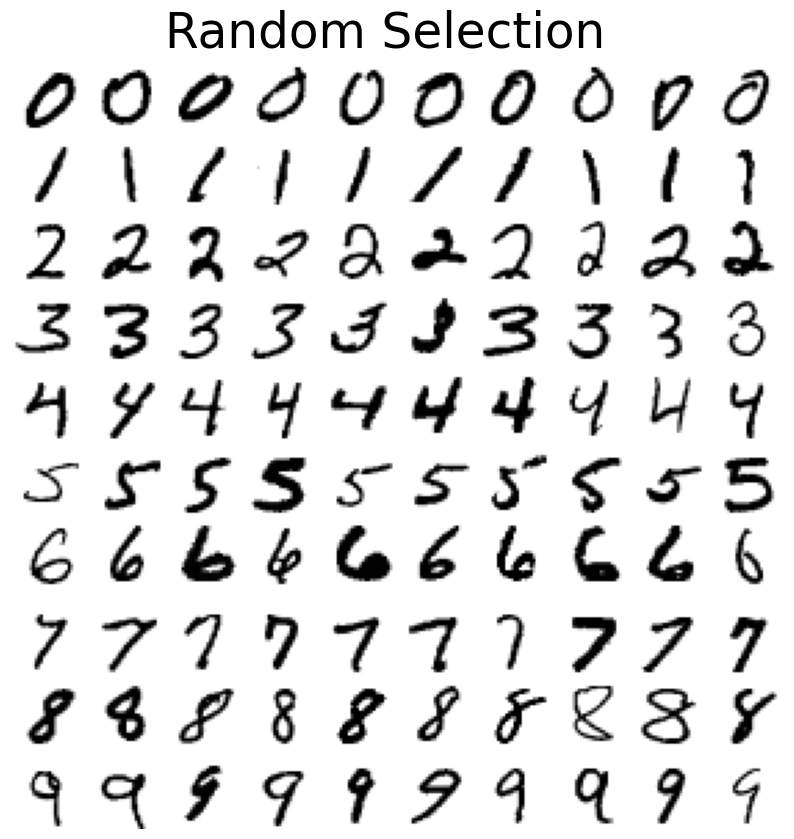
\includegraphics[width=\linewidth, trim={0 0 0 1.5cm},clip]{thesis_report/figures/mnist_inducing_point/random_mnist_inducing_point_selection.png}
\end{minipage}%
\begin{minipage}{.25\textwidth}
  \centering
  \textit{ARD}
  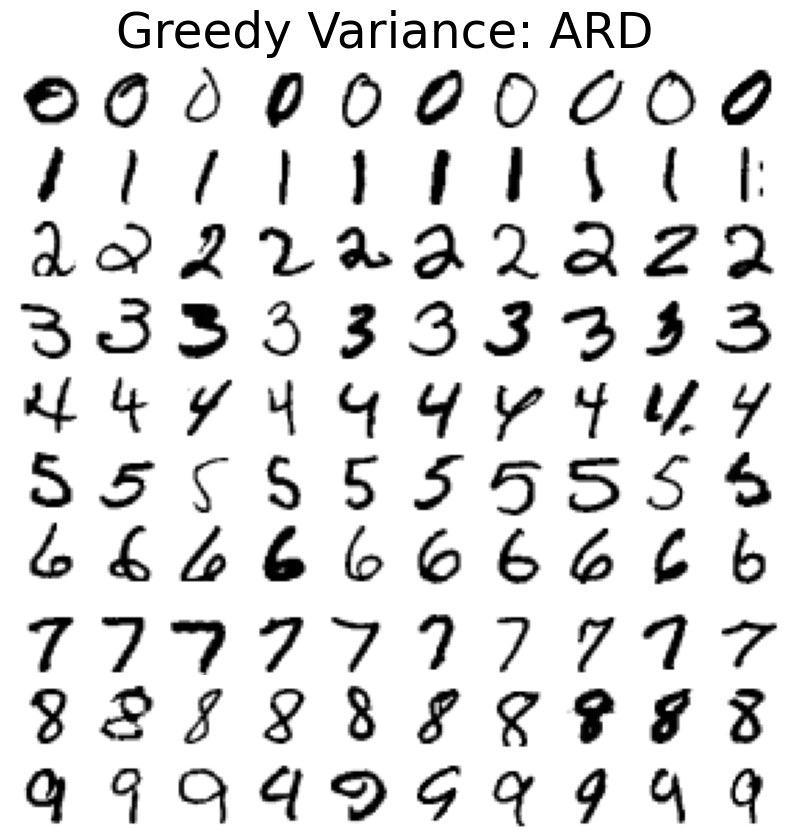
\includegraphics[width=\linewidth, trim={0 0 0 1.5cm},clip]{thesis_report/figures/mnist_inducing_point/greedy_mnist_ard_inducing_point_selection.png}
\end{minipage}%
\begin{minipage}{.25\textwidth}
  \centering
  \textit{FCNN NNGP}
  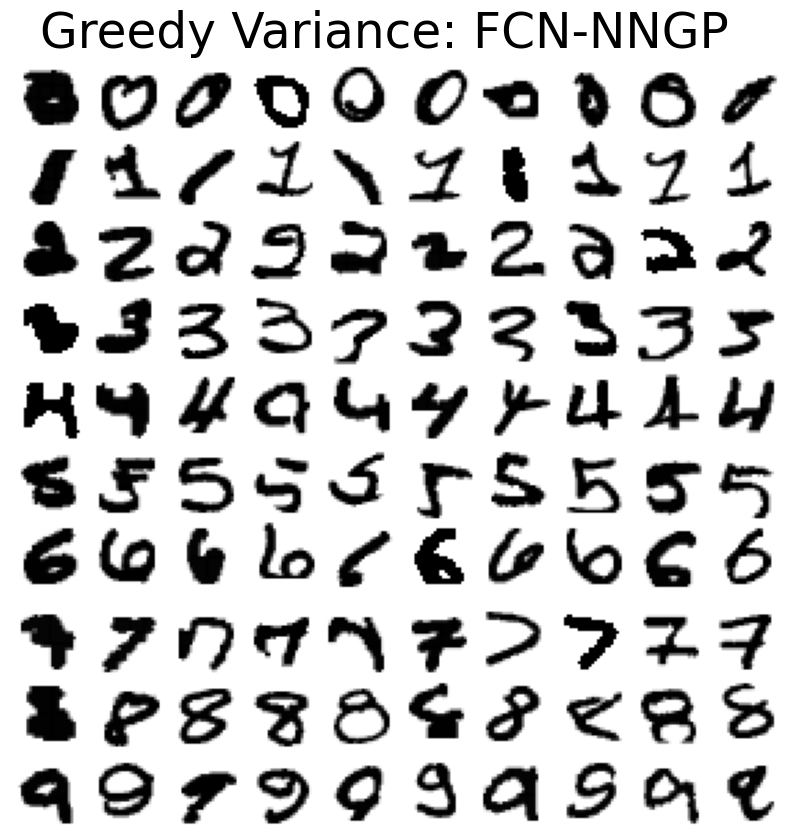
\includegraphics[width=\linewidth, trim={0 0 0 1.5cm},clip]{thesis_report/figures/mnist_inducing_point/greedy_mnist_fcn_nngp_inducing_point_selection.png}
\end{minipage}%
\begin{minipage}{.25\textwidth}
  \centering
  \textit{CNN NNGP}
  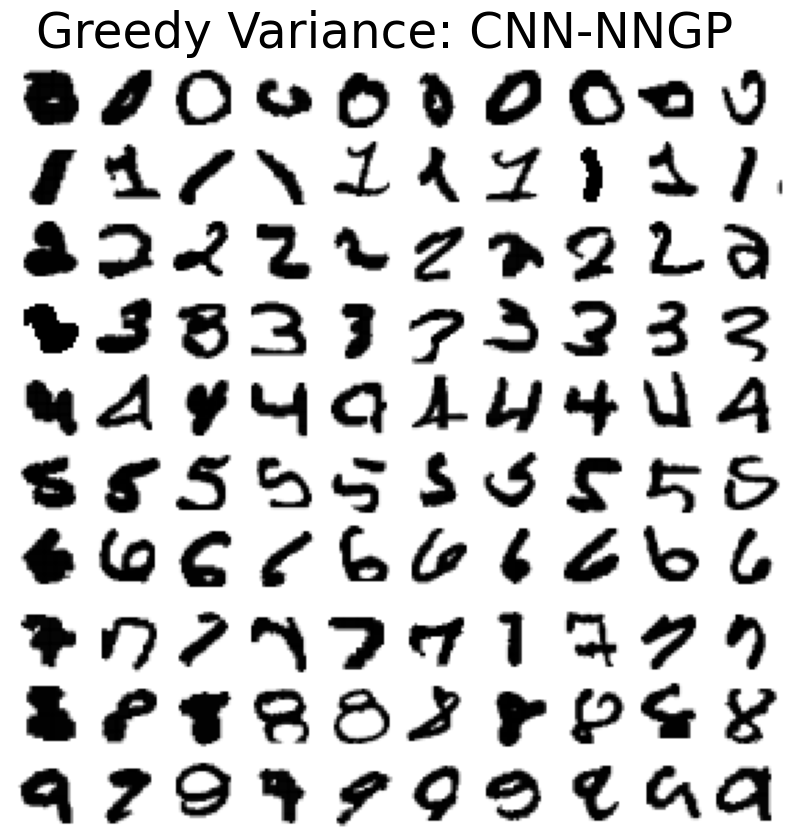
\includegraphics[width=\linewidth, trim={0 0 0 1.5cm},clip]{thesis_report/figures/mnist_inducing_point/greedy_mnist_cnn_nngp_inducing_point_selection.png}
\end{minipage}%
\caption{Inducing Point Selection with Different Kernels}\label{fig:mnist-inducing-points}
\end{figure}


\paragraph{Custom Feature Mapping Kernels} We also explored neural network kernels of the form
\begin{align}
    k(x, x') = k_0(h(x), h(x')),
    \label{custom-feature-map-kernel}
\end{align}
where $h: \mathcal{X} \rightarrow \mathbb{R}^D$ is a mapping to a $D$-dimensional feature space and $k_0: \mathbb{R}^D \times \mathbb{R}^D \rightarrow \mathbb{R}$ is a base kernel that can be any kernel function. 
We use Algorithm \ref{alg:inducing-points-prior-gp} to learn the hyper-parameters of $k_0$ and $h$. 
In our experiments, we chose non-stationary kernels for $k_0$ to ensure non-zero gradients for the gram matrix diagonals $k_0(h(x), h(x))$ with respect to the hyper-parameters of $h$. 
Like with NNGP kernels, we suggest choosing a suitable neural network architecture for $h$ depending on the data domain.

\begin{figure}[h!]
\small
\centering
\begin{minipage}{.25\textwidth}
  \centering
  \textit{FCNN Mapping}
  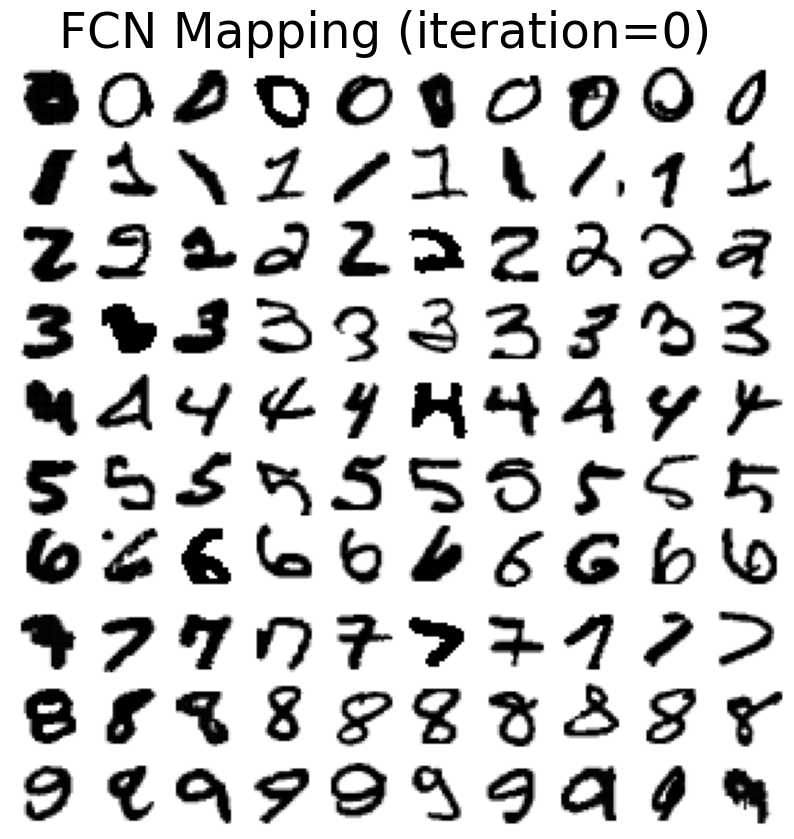
\includegraphics[width=\linewidth, trim={0 0 0 1.5cm},clip]{thesis_report/figures/custom_mapping/fcn/iteration_0.png}
\end{minipage}%
\begin{minipage}{.25\textwidth}
  \centering
  \textit{CNN Mapping}
  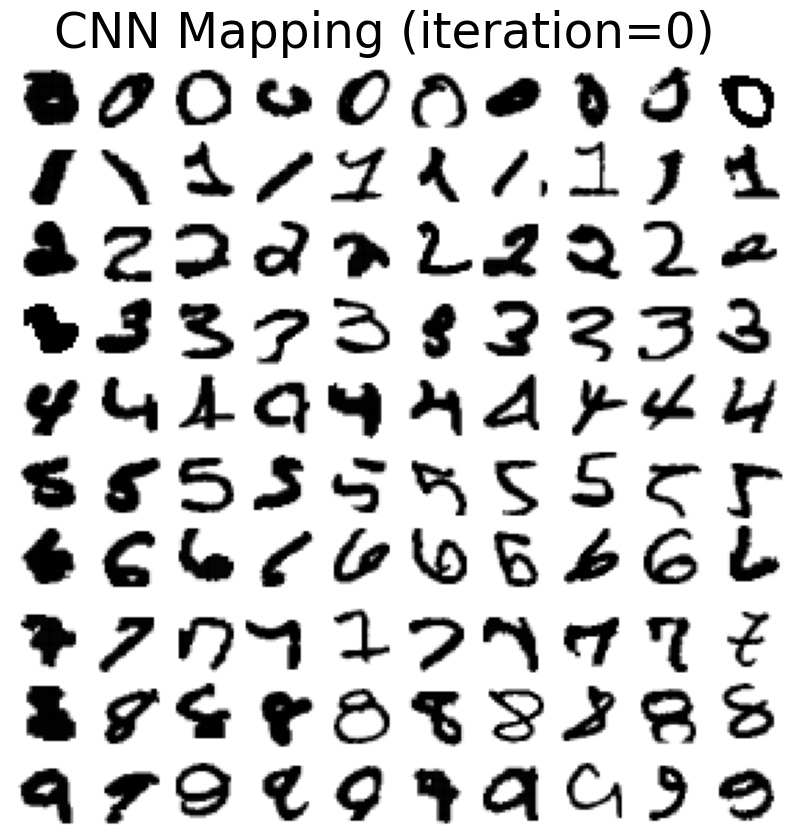
\includegraphics[width=\linewidth, trim={0 0 0 1.5cm},clip]{thesis_report/figures/custom_mapping/cnn/iteration_0.png}
\end{minipage}%
\caption{Inducing Point Selection with Randomly Initialised Feature Mapping Kernels}\label{fig:mnist-nn-mapping-kernels-0}
\end{figure}

\begin{figure}[h!]
\small
\centering
\begin{minipage}{.25\textwidth}
  \centering
  \textit{FCNN Mapping}
  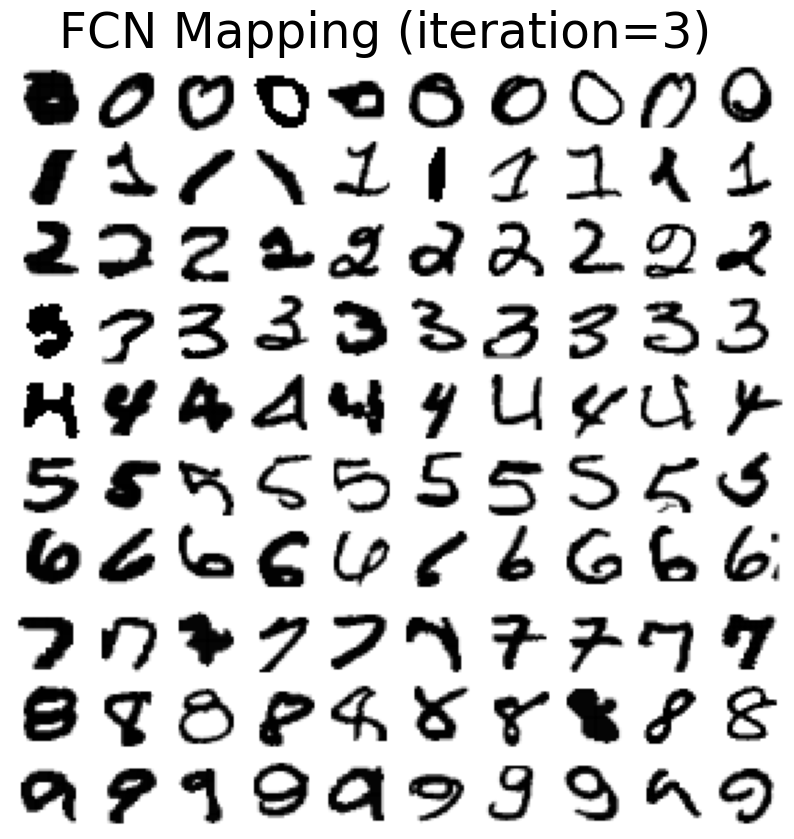
\includegraphics[width=\linewidth, trim={0 0 0 1.5cm},clip]{thesis_report/figures/custom_mapping/fcn/iteration_3.png}
\end{minipage}%
\begin{minipage}{.25\textwidth}
  \centering
  \textit{CNN Mapping}
  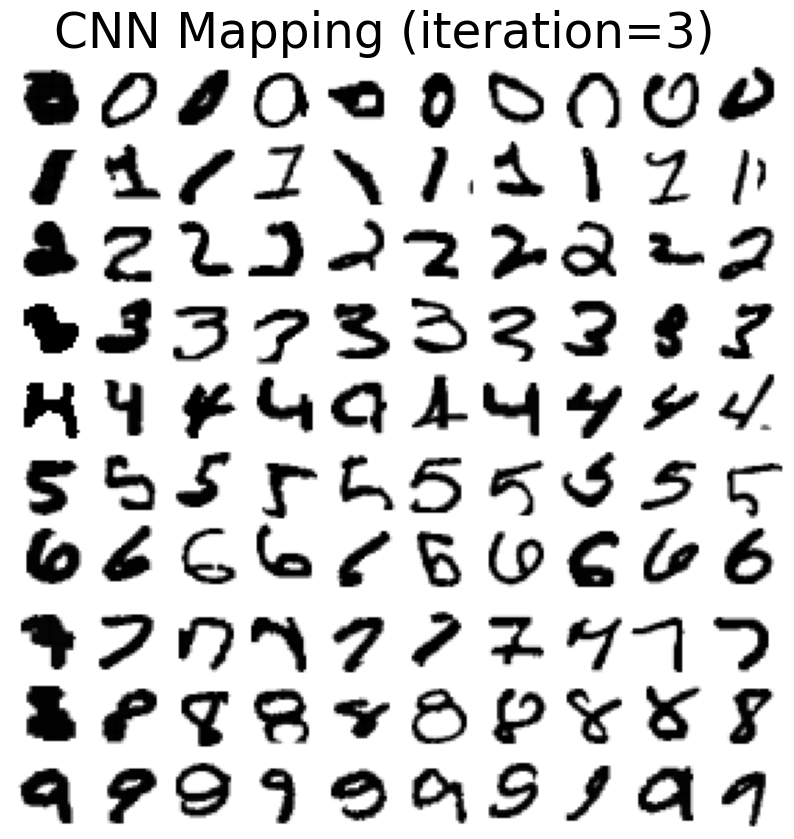
\includegraphics[width=\linewidth, trim={0 0 0 1.5cm},clip]{thesis_report/figures/custom_mapping/cnn/iteration_3.png}
\end{minipage}%
\caption{Inducing Point Selection with Trained Feature Mapping Kernels}\label{fig:mnist-nn-mapping-kernels-3}
\end{figure}

To motivate our approach, Figure \ref{fig:mnist-nn-mapping-kernels-0} shows inducing points selected with Algorithm \ref{alg:inducing-point-selection} using randomly initialised custom feature mapping kernels and selecting from the same 5000 images of each digit as for Figure \ref{fig:mnist-inducing-points}. 
We chose $k_0$ as a linear kernel and $h$ as a neural network (FCNN or CNN) with an output layer of $D=256$ features. 
We observed that even with random initialisation, the selected images are more diverse than the ARD kernel.
Figure \ref{fig:mnist-nn-mapping-kernels-3} visualises the inducing points after learning the hyper-parameters of $k$ with Algorithm \ref{alg:inducing-points-prior-gp}.
These images are qualitatively comparable to those selected by NNGP kernels.

\subsubsection{Variational Kernels}\label{variational-kernels}
The svGP kernel is given as
\begin{align}
    r(x, x') = k(x, x') - \mathbf{K}_{x, \mathbf{Z}} \mathbf{K}_{\mathbf{Z}, \mathbf{Z}} \mathbf{K}_{\mathbf{Z}, x'} + \mathbf{K}_{x, \mathbf{Z}} \mathbf{\Sigma} \mathbf{K}_{\mathbf{Z}, x'},
    \label{gwi-svgp-kernel}
\end{align}
where $\mathbf{\Sigma} \in \mathbb{R}^{M \times M}_{\succcurlyeq 0}$ is the hyper-parameter of $r$. 
\cite{wild2022generalized} proposes learning the positive semi-definite matrix $\mathbf{\Sigma}$ by learning the parameters of $\mathbf{L} \in \mathbb{R}^{M \times M}$, a lower triangle matrix with positive diagonal elements.
As a Cholesky decomposition, this ensures that $\mathbf{\Sigma} = \mathbf{L}\mathbf{L}^T \in \mathbb{R}^{M \times M}_{\succcurlyeq 0}$. 
We call this the Cholesky parameterisation. 
This section introduces new parameterisations for the svGP kernel followed by new forms of variational kernels.

\paragraph{svGP Parameterisations}
We introduce a new parameterisation of $\mathbf{\Sigma}$ called the diagonal parameterisation. The diagonal parameterisation learns
\begin{align}
    \diag(\mathbf{v}): \log(\mathbf{v}) \in \mathbb{R}^M,
\end{align}
where $\mathbf{\Sigma} = \diag(\mathbf{v}) \in \mathbb{R}^{M \times M}_{\succcurlyeq 0}$, a diagonal matrix of positive elements, and $\diag: \mathbb{R}^M \rightarrow \mathbb{R}^{M \times M}$, using a vector in $\mathbb{R}^M$ to construct a diagonal matrix in $\mathbb{R}^{M \times M}$.
Although this new parameterisation is more restrictive than the Cholesky parameterisation, it is computationally cheaper during gradient-based learning and has shown to have comparable performance during our experiments.

We also propose a base kernel parameterisation replacing $\mathbf{K}_{x, \mathbf{Z}} \mathbf{\Sigma} \mathbf{K}_{\mathbf{Z}, x}$, the last term of (\ref{gwi-svgp-kernel}) such that
\begin{align}
    r(x, x') = k(x, x') - \mathbf{K}_{x, \mathbf{Z}} \mathbf{K}_{\mathbf{Z}, \mathbf{Z}} \mathbf{K}_{\mathbf{Z}, x'} + r_0(x, x'),
\end{align}
where $r_0$ is the base kernel, which can be any kernel function. We learn the hyper-parameters of $r_0$ with GWI.

\paragraph{Sparse Posterior Kernels}
Inspired by the GP posterior covariance in (\ref{gp-posterior-covariance}) and the svGP kernel from \cite{titsias2009variational}, we present a new form of variational kernel we call sparse posterior kernels with the formulation
\begin{align}
    r(x, x') = r_0(x, x') - r_0\left(x, \mathbf{Z}\right) r_0\left(\mathbf{Z}, \mathbf{Z}\right)^{-1} r_0\left(\mathbf{Z}, x'\right),
\end{align}
where $r_0$ is any base kernel learned during GWI such that $r_0\left(x, \mathbf{Z}\right) \in \mathbb{R}^{1 \times M}$, $r_0\left(\mathbf{Z}, \mathbf{Z}\right) \in \mathbb{R}^{M \times M}$, and $r_0\left(\mathbf{Z}, x'\right) \in \mathbb{R}^{M \times 1}$ are gram matrices of $r_0$ following the construction in (\ref{gp-kernel-matrix}).
In our experiments, we chose $r_0$ as the same kernel as the prior kernel $k$. We also initialised its hyper-parameters with the hyper-parameters of $k$.
Treating $k\left(\mathbf{Z}, \mathbf{Z}\right)^{-1}$ as a pre-computed constant, sparse posterior kernels are $\mathcal{O}(M^2)$ to evaluate.

\paragraph{Fixed Sparse Posterior Kernels}
During GP prediction with sparse posterior kernels, the inversion $r_0\left(\mathbf{Z}, \mathbf{Z}\right)^{-1}$ is a constant. However during inference, gradients must pass through it to learn the parameters of the base kernel. Thus, we also present a fixed version of the sparse posterior kernel
\begin{align}
    r(x, x') = r_0(x, x') - r_0\left(x, \mathbf{Z}\right) k\left(\mathbf{Z}, \mathbf{Z}\right)^{-1} r_0\left(\mathbf{Z}, x'\right),
\end{align}
where the matrix inversion is a constant during inference and defined with respect to the prior kernel. This option provides faster training, no longer needing gradients to pass through a matrix inversion.

\subsection{An Improved Learning Procedure}
We improve on the GWI learning procedure from \cite{wild2022generalized} with Algorithm \ref{alg:gwi-gp}.
This algorithm abstracts the specific parameterisation of GWI-nets. 
It also includes an inducing point selection method, whereas \cite{wild2022generalized} selected inducing points randomly.
The rest of this section provides further details for certain steps of this procedure.
\begin{algorithm}[h!]
\caption{GWI-GP Learning}\label{alg:gwi-gp}
\begin{algorithmic}
    \Require{$k$, $m_Q$, $r$} \Comment{use zero mean for $m_P$}
    \State ($\theta$, $\mathbf{Z}$) $\leftarrow$ \Call{KernelAndInducingPoints}{$k$} \Comment{via Algorithm \ref{alg:inducing-points-prior-gp}, $\theta$ are hyper-parameters of $k$}
    \State $P \leftarrow$ ($k$, $\theta$) \Comment{construct prior/regulariser GP}
    \State $Q \leftarrow$ ($m_Q$, $r$, $\mathbf{Z}$) \Comment{construct GWI-GP}
    \State ($\gamma_{m_Q}$, $\gamma_r$) $\leftarrow$ \Call{OptimiseGWI}{$P$, $Q$} \Comment{via GWI, $\gamma_{m_Q}$, $\gamma_r$ are hyper-parameters of $m_Q$, $r$}
    \State $\gamma_r \leftarrow$ \Call{OptimiseTemper}{$\gamma_r$} \Comment{via type-II maximum likelihood on a validation set}
    \State \Return ($\gamma_{m_Q}$, $\gamma_r$)
\end{algorithmic}
\end{algorithm}
\paragraph{The Regulariser} The prior is an essential component of a Bayesian posterior belief update.
However in the context of GVI, the prior can be interpreted as a regulariser for empirical risk minimisation.
To prevent confusion in this discussion, we will call this the regulariser. 
In our experiments, we explored traditional regularisers constructed with the standard GP prior, having $\mathcal{O}(1)$ time complexity . 
Additionally, we propose another option for the GP regulariser
\begin{align}
    y \vert \mathbf{Z}, \mathbf{U}, \sigma^2
    \sim \mathcal{N}\left(\bar{m}_P(x), \bar{k}(x, x)\right),
    \label{gp-posterior-regulariser}
\end{align}
a `lightweight' Bayesian posterior using the inducing points $\mathbf{Z}\in \mathcal{X}^M$ and corresponding responses $\mathbf{U} \in \mathbb{R}^M$.
This regulariser would violate the traditional interpretation of a prior as it would explicitly use training data twice during inference.
However, we weaken this interpretation with the optimisation-centric nature of GVI, viewing this as a potentially better-informed regulariser than the unconditioned GP prior.
Our experiments show that this less-than traditional regulariser can sometimes construct a better learning objective for GWI-GPs.
Moreover, with inversions of $\mathbb{R}^{M\times M}$ matrices only, we maintain computational tractability when evaluating the GWI objective.
\newpage
\paragraph{Tempering}\cite{wild2022generalized} and \cite{adlam2020cold} explain that tempering the predictive posterior of GPs can improve predictive performance and has theoretical interpretations for correcting against a mis-specified prior. Following \cite{wild2022generalized}, we temper GWI-GPs by learning a factor $\alpha_T < 0$ for the tempered kernel formulated as
\begin{align}
    r_T(\mathbf{X}, \mathbf{X}) = \alpha_T \left(r(\mathbf{X}, \mathbf{X})+\sigma^2 \mathbf{I}\right),
\end{align}
where $\alpha_T$ is learned through negative log-likelihood optimisation on $Q\left(m_Q, r_T\right)$ with a hold-out validation set. 
The rest of the GP hyper-parameters are held fixed during this process. 
This forms the final GWI-GP such that the predictive posterior is given as
\begin{align}
    y \sim \mathcal{N}\left(m_Q(x), \alpha_T \left( r(x, x) + \sigma^2\right) \right).
\end{align}
Tempering is also applied to classification by constructing $\left[\alpha_T^1 \dots \alpha_T^J\right]^T \in [0, \infty)^J$, a separate tempering factor for each GP, and optimising the classification log-likelihood in (\ref{robust-max-function-expected-log-likelihood}).


\begin{figure}[h!]
\small
\centering
\begin{minipage}{.5\textwidth}
  \centering
  \textit{Untempered}
  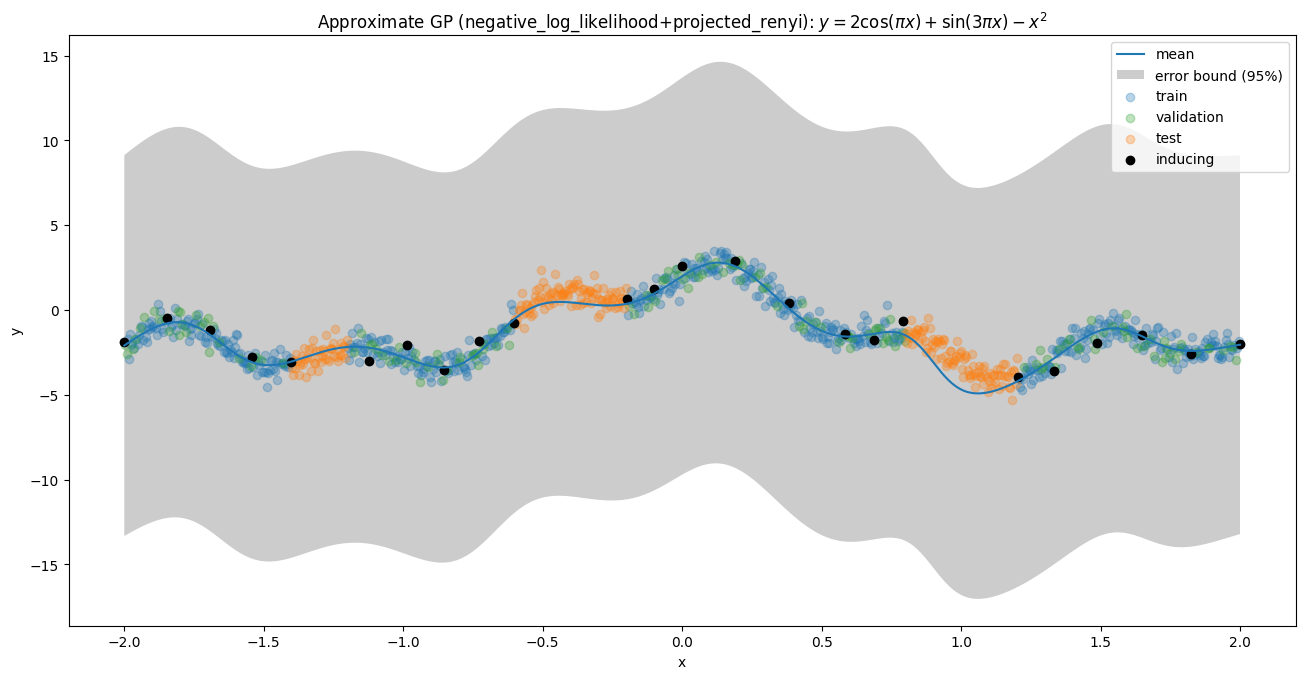
\includegraphics[width=\linewidth, trim={0 0 0 0.84cm},clip]{thesis_report/figures/tempering/untempered.png}
\end{minipage}%
\begin{minipage}{.5\textwidth}
  \centering
  \textit{Tempered}
  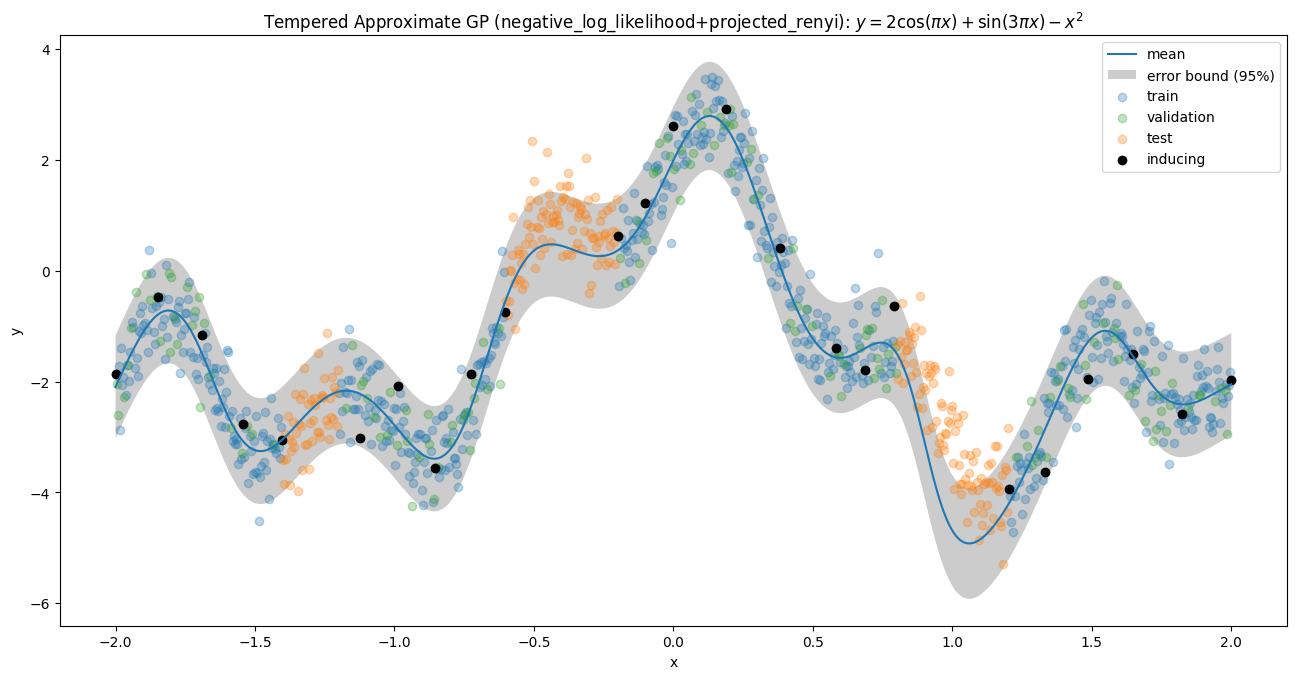
\includegraphics[width=\linewidth, trim={0 0 0 0.85cm},clip]{thesis_report/figures/tempering/tempered.png}
\end{minipage}%
\caption{Tempering the GWI-GP \textit{(black inducing points, blue training points, green validation points, and orange test points)}}
\label{fig:tempered-gwi}
\end{figure}

Figure \ref{fig:tempered-gwi} visualises an extreme example of a GP before and after tempering. We observe that $\alpha_T$ is essentially `squeezing' the variance to more appropriate uncertainty bounds for the data, while the rest of the GP's behaviour remains the same.


\subsection{Wasserstein Distance Approximations}
\cite{wild2022generalized} provides the batched approximation of the Wasserstein distance from (\ref{wasserstein-distance}) for $N$ data points as
\begin{align}
    \mathbb{W}\left[Q, P\right]^2  &\approx \frac{1}{N_B}\sum_{n_b=1}^{N_B} \left(m_P(x_{n_b}) - m_Q(x_{n_b})\right)^2 \nonumber \\
    & \qquad + \frac{1}{N_B} \sum_{n_b=1}^{N_B} k(x_{n_b}, x_{n_b}) + \frac{1}{N_B} \sum_{n_b=1}^{N_B} r(x_{n_b}, x_{n_b}) \nonumber \\
    & \qquad - \frac{2}{\sqrt{N_B N_S}} \sum_{n_s=1}^{N_S} \sqrt{\lambda_{n_s}\left\big(r\left(\mathbf{X}_{N_S}, \mathbf{X}_{N_B}\right)k\left(\mathbf{X}_{N_B}, \mathbf{X}_{N_S}\right)\right\big)},
    \label{wasserstein-distance-approximation}
\end{align}
where $N_B < N$ and $N_S < N$ for two independent batches and $\lambda_{n}(\cdot)$ evaluates the $n^{th}$ eigenvalue. We introduce further numerical approximations of (\ref{wasserstein-distance-approximation}) to improve computation speed.

\paragraph{Symmetric Matrices}In our experiments, we use the same data sample for $\mathbf{X}_{N_B}$ and $\mathbf{X}_{N_S}$, to ensure symmetric square matrices for $r\left(\mathbf{X}_{N_S}, \mathbf{X}_{N_B}\right)$ and $k\left(\mathbf{X}_{N_B}, \mathbf{X}_{N_S}\right)$ in the eigendecomposition term of (\ref{wasserstein-distance-approximation}). 
This allows us to take advantage of eigenvalue properties of symmetric matrices, further explained in Appendix \ref{appendix:eigenvalue-symmetric-matrix}. 
We use symmetric matrices to leverage the eigendecomposition implementation in version 0.4 of Python JAX, which is only available on GPUs for symmetric matrices. 
Our experiments showed that using the same batch for $\mathbf{X}_{N_S}$ and $\mathbf{X}_{N_B}$ doesn't seem to make any significant difference on the resulting GWI-GP.

\paragraph{Dropping the Eigendecomposition}The eigendecomposition in the last term of (\ref{wasserstein-distance-approximation}) is computationally expensive with $\mathcal{O}(N^3)$ complexity, which in our case is the sample size $N_S$.
In our GWI experiments we often dropped this term with negligible practical effects.
This imprecise regulariser, which caused minimal change to our inference results, was significantly counteracted by much faster training speeds.

\newpage
\section{Projected Generalised Variational Inference for Gaussian Processes}\label{section:pgvi}
This section proposes projected GVI (pGVI) for GPs, a new framework to learn variational GPs that we call pGVI-GPs.
pGVI uses the same learning procedure in Algorithm \ref{alg:gwi-gp}, except it replaces the Wasserstein regularisation with a new form of regularisation that we call projected regularisation.
Projected regularisations are computationally cheap, making pGVI an extremely attractive option in practice.
We will present the general projected regularisation formulation followed by different constructions of the pGVI objective.

\subsection{Projected Regularisation}
The GVI framework from \cite{knoblauch2022optimization} assumes
\begin{align}
    \mathbb{D}\left[Q, P\right] = 0 \Leftrightarrow P = Q,
\end{align}
in other words, that the regulariser $\mathbb{D}$ is definite.
We weaken this assumption and propose regularisers of the form
\begin{align}
    \mathbb{D}\left[Q, P\right] = \frac{1}{N}\sum_{{n}=1}^{N} \mathbb{D}_0 \Big[\mathbb{Q}\left(F(x_n)\right), \mathbb{P}\left(F(x_n)\right)\Big],
    \label{proj-regulariser}
\end{align}
where $\mathbb{D}_0$ is a (base) regulariser between two probability measures on $\mathbb{R}$ and $x_n \in \mathcal{X}$.
Specifically, since both the variational approximation and regulariser are GPs, we have that $\mathbb{Q}\left(F(x_n)\right) = \mathcal{N}\left(m_Q(x_n), r(x_n, x_n)\right)$ and $\mathbb{P}\left(F(x_n)\right) = \mathcal{N}\left(m_P(x_n), k(x_n, x_n)\right)$.
Therefore any base regulariser $\mathbb{D}_0$ that can be computed between two scalar Gaussian random variables will lead to a tractable regulariser computation and therefore a tractable variational loss. We call regularisation schemes following (\ref{proj-regulariser}), projected regularisation.

Projected regularisations were inspired by the experimental observation that dropping the eigendecomposition in the GWI objective (\ref{wasserstein-distance-approximation}) had negligible effect on the training procedure.
By only regularising against the marginal function values in (\ref{proj-regulariser}), we are similarly unconstrained with respect to correlations.
However our experiments show that this can be a sufficient regulariser to recover most of the benefits of GVI in terms of uncertainty quantification. 
This suggests that in practice, the assumption of a definite regulariser may sometimes be overly strict.
% In most practical VI use cases where $Q$ is an approximation, we would rarely expect to actually be in a setting where $Q$ matches our target posterior. \vw{I think you dont need the previous sentence. Your point still holds without it and it is probably a bit controversial to say this.}
The experimental success of projected regularisation suggests that a regulariser $\mathbb{D}[Q, P] \geq 0$ having capacity to prevent overfitting to the empirical risk may be sufficient to provide a reasonable learning objective for GVI.


The experimentally-driven approach of pGVI is attractive because it is computationally cheaper than GWI or any other previous approaches to function space VI.
The base regularisers that we propose have $\mathcal{O}(1)$ time complexity  with respect to a training input $x_n$.
For a batch of $N_B$ points we have $\mathcal{O}(N_B)$, much faster than $\mathcal{O}(N_B^3)$ for the Wasserstein distance in (\ref{wasserstein-distance-approximation}).  
Other approaches like \cite{rudner2020rethinking}, \cite{sun2019functional}, \cite{ma2019variational}, and \cite{ma2021functional} generally attempt to stochastically approximate a function space KL divergence with some finite $N$-dimensional realisation, also having complexity $\mathcal{O}(N_B^3)$. 
This makes the linear time complexity of pGVI an extremely attractive approach in practice.

\subsection{Base Regularisers}
We now review the base regularisers $\mathbb{D}_0$ used in our experiments. 
These provide different constructions of the pGVI objective, demonstrating the modularity of our approach.
In the following, we denote $Q_{x} \coloneqq \mathbb{Q}\left(F(x)\right)$, $P_{x} \coloneqq \mathbb{P}\left(F(x)\right)$, $\mu_p \coloneqq m_P(x)$, $\mu_q \coloneqq m_Q(x)$, $\sigma_p^2 \coloneqq k(x, x)$, and $\sigma_q^2 \coloneqq r(x, x)$.
\paragraph{The Bhattacharyya distance} Given as
\begin{align}
    \mathbb{B} \left[Q_{x}, P_{x}\right] &= \frac{1}{4} \frac{\left(\mu_p - \mu_q\right)^2}{\sigma_p^2 + \sigma_q^2} + \frac{1}{2} \log\left(\frac{\sigma_p^2 + \sigma_q^2}{2\sigma_p\sigma_q^}\right).
\end{align}
\paragraph{The Wasserstein distance} Given as
\begin{align}
    \mathbb{W} \left[Q_{x}, P_{x}\right]^2 &= \left(\mu_p - \mu_q\right)^2 + \sigma_p^2 + \sigma_q^2 - 2 \sigma_p\sigma_q
\end{align}
for Gaussians on $\mathbb{R}$.
\paragraph{The Hellinger divergence} Given as
\begin{align}
    \mathbb{H} \left[Q_{x}, P_{x}\right] = 1 - \sqrt{\frac{2\sigma_p\sigma_q}{\sigma_p^2 + \sigma_q^2}} \exp\left(-\frac{1}{4} \frac{ \left(\mu_p - \mu_q\right)^2}{\sigma_p^2 + \sigma_q^2}\right).
\end{align}
\paragraph{The KL divergence} Given as
\begin{align}
    \mathbb{KL} \left[Q_{x}, P_{x}\right] &= \log\frac{\sigma_q}{\sigma_p} + \frac{\sigma_p^2 + \left(\mu_p - \mu_q\right)^2}{2 \sigma_q^2} - \frac{1}{2}
\end{align}
for Gaussian on $\mathbb{R}$.
\paragraph{The $\alpha$-Renyi divergence} Given as
\begin{align}
    \mathbb{R}_\alpha \left[Q_{x}, P_{x}\right] &= \log\frac{\sigma_p}{\sigma_q} + \frac{1}{2(\alpha-1)}\log\left(\frac{\sigma_p^2}{\alpha \sigma_p^2 + (1-\alpha) \sigma_q^2}\right)  + \frac{1}{2}\frac{\alpha \left(\mu_p - \mu_q\right)^2}{\alpha \sigma_p^2 + (1-\alpha) \sigma_q^2},
\end{align}
with $\alpha \sigma_p^2 + (1-\alpha) \sigma_q^2 > 0$.
\paragraph{A naive divergence}Finally, we also experimented with a naive divergence
\begin{align}
    \mathbb{N} \left[Q_{x}, P_{x}\right] = \left(\mu_p - \mu_q\right)^2 + \left(\sigma_q^2-\sigma_p^2\right)^2,
\end{align}
combining the squared difference of the means and covariances.

\newpage
\section{Experimentation Framework}\label{section:experimentation-framework}
This section presents the experimentation framework that we developed for GWI-GPs and pGVI-GPs.
We begin by summarising our implementation architecture followed by a description of our experimentation setup.
Lastly, we will present results for some 1-D regression problems to show our framework in action.
Our Python implementation is openly available on \href{https://github.com/jswu18/gvi-gaussian-process}{GitHub}\footnote{For the most up-to-date version, see: \href{https://github.com/jswu18/gvi-gaussian-process}{https://github.com/jswu18/gvi-gaussian-process}}$^{,}$\footnote{
For the last version prior to the submission date, see: \\\href{https://github.com/jswu18/gvi-gaussian-process/tree/a24dd7188f51e06b3e7dca4e2a4847ba05e0f62a}{https://github.com/jswu18/gvi-gaussian-process/tree/a24dd7188f51e06b3e7dca4e2a4847ba05e0f62a}}. 
It should be noted that our implementation collects the terms svGP, GWI-GP, and pGVI-GP under the umbrella name `approximate GP'.

\subsection{Implementation Architecture}\label{implementation-architecture}
GWI and pGVI are both highly flexible learning frameworks. 
As such, abstraction was critical for ensuring scaleable and maintainable implementations.
Luckily, the GVI framework proposed by \cite{knoblauch2022optimization} naturally translates to an architecture that we outline with the UML class diagram in Figure \ref{gvi-implementation}.
For visual clarity, we only included relevant attributes and methods.
We see that the GVI objective in (\ref{gvi-posterior-in-fs}) with $\ell$ and $\mathbb{D}$ has been abstracted to accommodate any valid empirical risk and regularisation, respectively.
These abstractions are exactly mirrored in our implementation architecture as abstract base classes, ensuring that the same interface is maintained for all child classes.
\begin{figure}[h!]
\begin{center}
\resizebox{\textwidth}{!}{
\begin{tikzpicture}

\begin{class}[text width=5cm]{GVI}{0,0}
\attribute{empirical risk : EmpiricalRisk}
\attribute{regularisation : Regularisation}
\operation{calculate ( $\gamma$ , $\mathbf{X}$ , $\mathbf{Y}$ ) : float}
\end{class}

\begin{abstractclass}[text width=5cm]{EmpiricalRisk}{-6,-3}
\attribute{$Q$ : ApproximateGP}
\operation{calculate ( $\gamma$ , $\mathbf{X}$ , $\mathbf{Y}$ ) : float}
\end{abstractclass}


\begin{class}[text width=5cm]{NegativeLogLikelihood}{-9,-6}
\inherit{EmpiricalRisk}
\end{class}

\begin{class}[text width=5cm]{CrossEntropy}{-3,-6}
\inherit{EmpiricalRisk}
\end{class}

\begin{abstractclass}[text width=5cm]{Regularisation}{6 , -3}
\attribute{$P$ : ExactGP}
\attribute{$\theta$ : ExactGP Parameters}
\attribute{$Q$ : ApproximateGP}
\attribute{mode : \{`prior', `posterior'\}}
\operation{calculate ( $\gamma$ , $\mathbf{X}$ ) : float}
\end{abstractclass}

\begin{class}[text width=5cm]{Wasserstein}{9,-7.5}
\inherit{Regularisation}
\attribute{include eigendecomp. : bool}
\end{class}

\begin{abstractclass}[text width=5cm]{ProjectedRegularisation}{0,-7.5}
\inherit{Regularisation}
\end{abstractclass}

\begin{class}[text width=5cm]{Bhattacharyya}{-9,-9.25}
\inherit{ProjectedRegularisation}
\end{class}

\begin{class}[text width=5cm]{Wasserstein}{-9,-11}
\inherit{ProjectedRegularisation}
\end{class}

\begin{class}[text width=5cm]{Hellinger}{-3,-11}
\inherit{ProjectedRegularisation}
\end{class}

\begin{class}[text width=5cm]{KL}{3,-11}
\inherit{ProjectedRegularisation}
\end{class}

\begin{class}[text width=5cm]{Renyi}{9,-11}
\inherit{ProjectedRegularisation}
\attribute{$\alpha$ : float}
\end{class}

\begin{class}[text width=5cm]{SquaredDifference}{9,-9.25}
\inherit{ProjectedRegularisation}
\end{class}

\composition{GVI}{}{}{EmpiricalRisk}
\composition{GVI}{}{}{Regularisation}

\end{tikzpicture}
}
\caption{UML Class Diagram of the GVI Implementation Architecture}
\label{gvi-implementation}
\end{center}
\end{figure}

Algorithms \ref{alg:inducing-point-selection}, \ref{alg:inducing-points-prior-gp}, and \ref{alg:gwi-gp} are abstracted for any mean, kernel, and variational kernel. We developed the architecture in Figure \ref{gp-implementation} for our implementation of GPs, Figure \ref{mean-implementation} for mean functions, and Figure \ref{kernel-implementation} for kernels. 
These architectures are also exactly reflected in our code base.
\begin{figure}[h!]
\begin{center}
\resizebox{\textwidth}{!}{
\begin{tikzpicture}

\begin{abstractclass}[text width=5cm]{GP}{0, 4}
\attribute{$m$ : Mean}
\attribute{$k$ : Kernel}
\end{abstractclass}

\begin{abstractclass}[text width=5cm]{ExactGP}{-9, 1.25}
\inherit{GP}
\attribute{$\mathbf{X}$ : array}
\attribute{$\mathbf{Y}$ : array}
\operation{predict ( $\theta$ , $x$ ) : Distribution}
\end{abstractclass}

\begin{abstractclass}[text width=5cm]{GPRegression}{-3, 1.25}
\inherit{GP}
\attribute{dist. : Dist. = Gaussian}
\end{abstractclass}

\begin{abstractclass}[text width=5cm]{GPClassification}{3, 1.25}
\inherit{GP}
\attribute{dist. : Dist = Multinomial}
\end{abstractclass}

\begin{abstractclass}[text width=5cm]{ApproxGP}{9, 1.25}
\inherit{GP}
\operation{predict ( $\gamma$ , $x$ ) : Distribution}
\end{abstractclass}

\begin{class}[text width=5cm]{ExactGPRegression}{-9, -3}
\inherit{ExactGP}
\inherit{GPRegression}
\end{class}

\begin{class}[text width=5cm]{ApproxGPRegression}{-3, -3}
\inherit{ApproxGP}
\inherit{GPRegression}
\end{class}

\begin{class}[text width=5cm]{ExactGPClassification}{3, -3}
\inherit{ExactGP}
\inherit{GPClassification}
\end{class}

\begin{class}[text width=5cm]{ApproxGPClassification}{9, -3}
\inherit{ApproxGP}
\inherit{GPClassification}
\end{class}


\begin{abstractclass}[text width=5cm]{Mean}{-9, 3.85}
\operation{predict ( $\theta_{m}$ , $x$ ) : array}
\end{abstractclass}

\begin{abstractclass}[text width=5cm]{Kernel}{9, 3.85}
\operation{gram ( $\theta_{k}$ , $x$ ) : array}
\end{abstractclass}

\composition{GP}{}{}{Mean}
\composition{GP}{}{}{Kernel}
\end{tikzpicture}
}
\caption{UML Class Diagram of the GP Implementation Architecture}
\label{gp-implementation}
\end{center}
\end{figure}


\begin{figure}[h!]
\begin{center}
\resizebox{0.75\textwidth}{!}{
\begin{tikzpicture}
\begin{abstractclass}[text width=5cm]{Mean}{0, 0}
\operation{predict ( $\theta_{m}$ , $x$ ) : array}
\end{abstractclass}

\begin{class}[text width=5cm]{Constant}{0, -3}
\inherit{Mean}

\end{class}
\begin{class}[text width=5cm]{SVGP}{-6, -3}
\attribute{$m_P$ : Mean}
\attribute{$\theta_{m_P}$ : Mean Parameters}
\attribute{$k$ : Kernel}
\attribute{$\theta_{k}$ : Kernel Parameters}
\attribute{$\mathbf{Z}$ : array}
\inherit{Mean}
\end{class}

\begin{class}[text width=5cm]{NeuralNetwork}{6, -3}
\attribute{architecture : list}

\inherit{Mean}
\end{class}
\end{tikzpicture}
}
\caption{UML Class Diagram of the Mean Function Implementation Architecture}
\label{mean-implementation}
\end{center}
\end{figure}



\begin{figure}[h!]
\begin{center}
\resizebox{\textwidth}{!}{
\begin{tikzpicture}
\begin{abstractclass}[text width=5cm]{Kernel}{4, 0}
\operation{gram ( $\theta_{k}$ , $x$ ) : array}
\end{abstractclass}

\begin{class}[text width=5cm]{Polynomial}{-2, -1.5}
\attribute{degree : float}
\inherit{Kernel}
\end{class}

\begin{class}[text width=5cm]{ARD}{-2, -4}
\inherit{Kernel}
\end{class}

\begin{class}[text width=5cm]{CustomFeatureMapping}{10, -4}
\attribute{$k_0$ : Kernel}
\attribute{$h$ : NeuralNetwork}
\inherit{Kernel}
\end{class}

\begin{class}[text width=5cm]{NNGP}{10, -1.5}
\attribute{architecture: list}
\inherit{Kernel}
\end{class}

\begin{abstractclass}[text width=5cm]{Approximate}{4, -4}
\inherit{Kernel}
\attribute{$\mathbf{Z}$ : array}
\end{abstractclass}

\begin{abstractclass}[text width=5cm]{SVGP}{1, -7}
\inherit{Approximate}
\attribute{$k$ : Kernel}
\attribute{$\theta_{k}$ : Kernel Parameters}
\end{abstractclass}

\begin{class}[text width=5cm]{SparsePosterior}{7, -7}
\inherit{Approximate}
\attribute{$r_0$ : Kernel}
\end{class}

\begin{class}[text width=5cm]{FixedSparsePosterior}{13, -7}
\inherit{Approximate}
\attribute{$k$ : Kernel}
\attribute{$\theta_{k}$ : Kernel Parameters}
\attribute{$r_0$ : Kernel}
\end{class}

\begin{class}[text width=5cm]{CholeskySVGP}{-5, -10.5}
\inherit{SVGP}
\end{class}

\begin{class}[text width=5cm]{DiagonalSVGP}{1, -10.5}
\inherit{SVGP}
\end{class}

\begin{class}[text width=5cm]{KernelisedSVGP}{7, -10.5}
\attribute{$r_0$ : Kernel}
\inherit{SVGP}
\end{class}

\end{tikzpicture}
}
\caption{UML Class Diagram of the Kernel Function Implementation Architecture}
\label{kernel-implementation}
\end{center}
\end{figure}

Our implementation is in Python and predominantly uses JAX, a high-performance numerical computing package developed by \cite{jax2018github}.
Because there is currently no existing stable, well-maintained, and well-documented implementation of GPs using JAX, we developed many of our implementations from scratch.
We chose JAX for its currently growing user-base, unique customisations, and to ensure compatibility with the implementation of NNGP kernels by \cite{novak2019neural}, which is also developed in JAX.
We chose Python for its current popularity within the machine learning community.
We also incorporated a number of commonly used implementation techniques whenever necessary, such as adding jitter and using the Cholesky decomposition for matrix inversions.

We use a number of standard software engineering tools to ensure a scaleable, maintainable, and controlled environment for our growing code base.
We introduced strict typing controls for all model parameter classes with Pydantic base models from \cite{samuel_colvin_2023_8277473}.
Pydantic models enforce typing hints during run-time that would otherwise be considered `syntactic sugar' in Python. This also provides clear guidelines when constructing models within our implementation framework.
We also included a rigorous number of tests that currently has 95\% test coverage over the implementations found in the \code{src/} directory, much higher than needed in most software development projects.
This also includes the use of mockers for isolated testing environments of different components (i.e. mean and kernel mockers to isolate testing of GP implementations). 
Finally, we use Poetry developed by \cite{Eustace} to strictly control package requirements, ensuring the version compatibility of dependencies.

\subsection{Experiment Scaling}
In addition to our implementation architecture, we developed a scaleable approach to experimentation.
Implemented in the \code{experiments/} directory, we constructed schemas and resolvers for each abstraction that we described in Section \ref{implementation-architecture}.
This allowed us to define and construct experiments through \code{.yaml} configuration files.
Each \code{.yaml} outlines the settings of an experiment (the GP, learning objective, learning rate, optimiser, etc.).
Appendix \ref{appendix:configuration-yamls} shows example \code{.yaml} configuration files for training a regulariser GP and an approximate GP .

Generating configuration files was automated, allowing us to scale our experiments to all possible combinations of empirical risks, regularisers, mean functions, and kernels. 
These configurations were then submitted as jobs to a computing cluster, running our experiments in an organised and well-documented environment.

\subsection{Regression Curve Experiments}
To demonstrate our experimentation framework, we trained approximate GPs for ten different regression curve problems. 
Randomly selected segments of each curve were removed from the training data to simulate an out-of-distribution (OOD) setting.
% We also explored two settings, a less aggressive setting where about a quarter of the training data is removed, and a more aggressive setting where about half is removed. 
% We did this to explore the effects of different out-of-distribution (OOD) settings.

Using our framework, we constructed 1260 combinations of experiment settings, each defined through \code{.yaml} configuration files. 
Each setting includes a unique combination of constructions for the regulariser GP, the approximate GP, and the GVI objective, among other parameters. 
The lists of options for each section that we explored are outlined in Appendix \ref{appendix:configurations}.
After running all 1260 combinations, we selected the experiment having the best validation set negative log-likelihood. 

\newpage
\begin{figure}[h!]
\centering
\small
\begin{minipage}{.5\textwidth}
  \centering
  \textit{Curve 1}
  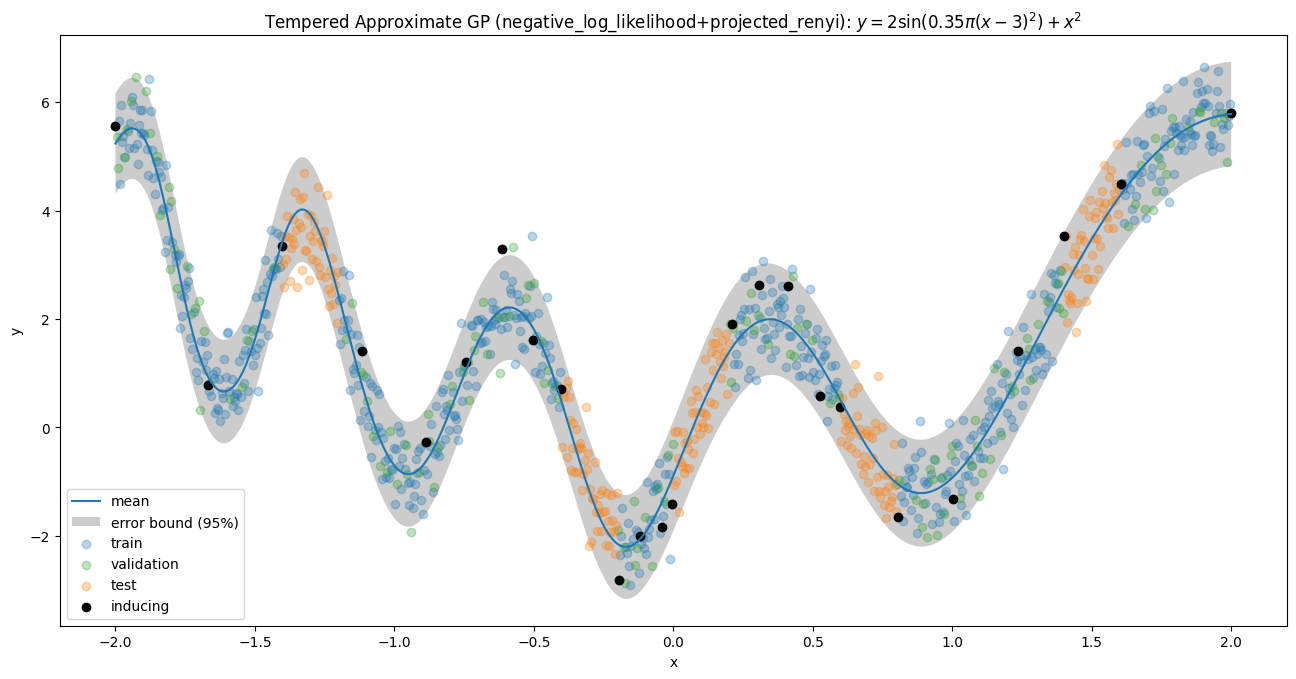
\includegraphics[width=\linewidth, trim={0 0 0 0.885cm},clip]{thesis_report/figures/toy_curves/curve0.png}
  \textit{Curve 3}
  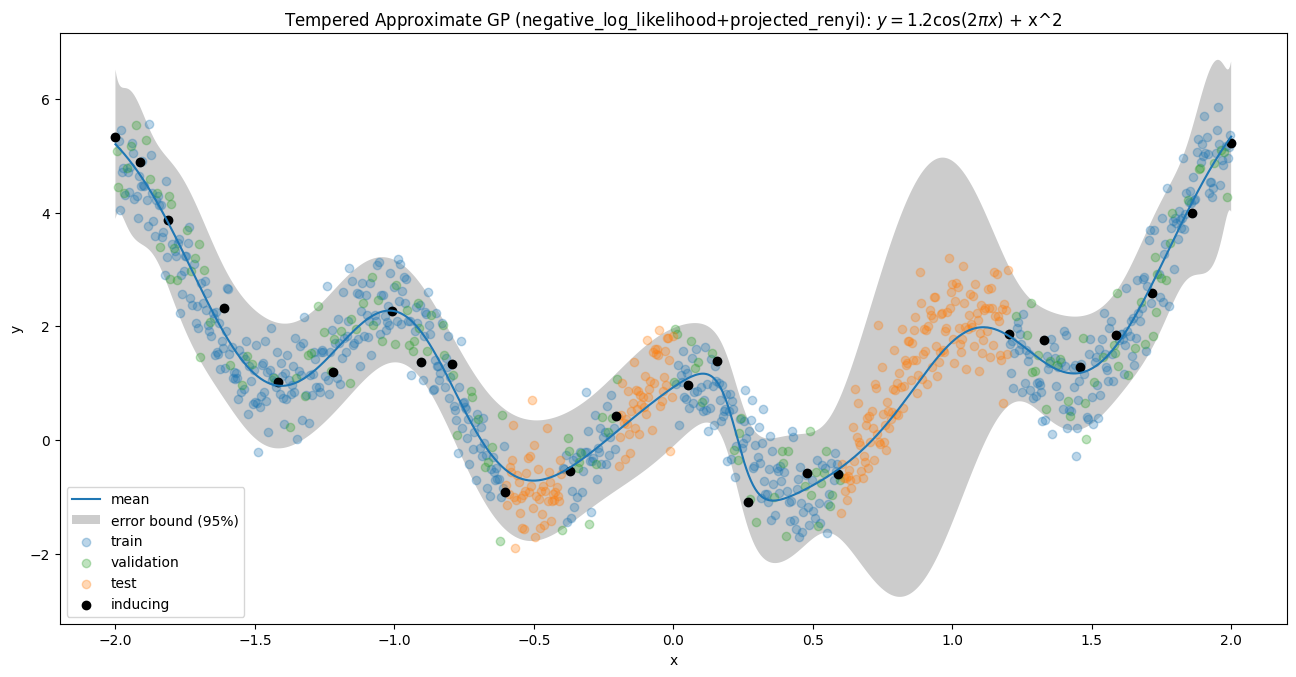
\includegraphics[width=\linewidth, trim={0 0 0 0.82cm},clip]{thesis_report/figures/toy_curves/curve2.png}
  \textit{Curve 5}
  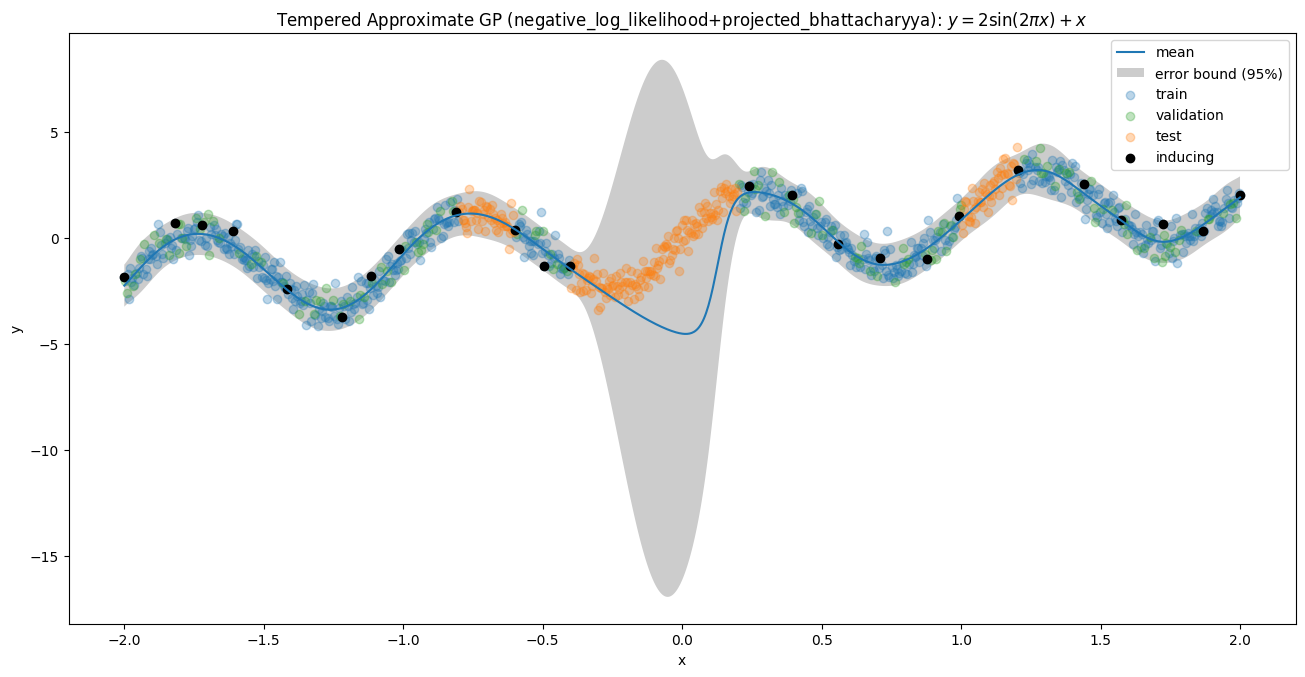
\includegraphics[width=\linewidth, trim={0 0 0 0.8cm},clip]{thesis_report/figures/toy_curves/curve4.png}
  \textit{Curve 7}
  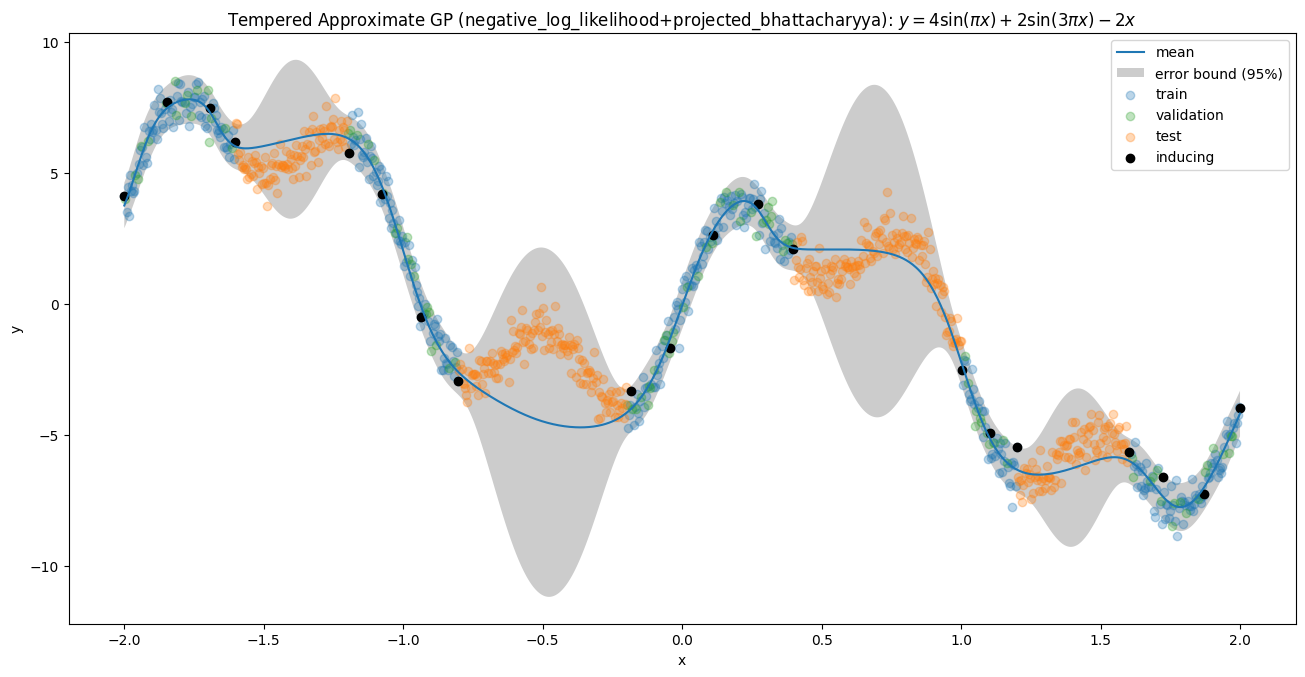
\includegraphics[width=\linewidth, trim={0 0 0 0.8cm},clip]{thesis_report/figures/toy_curves/curve6.png}
  \textit{Curve 9}
  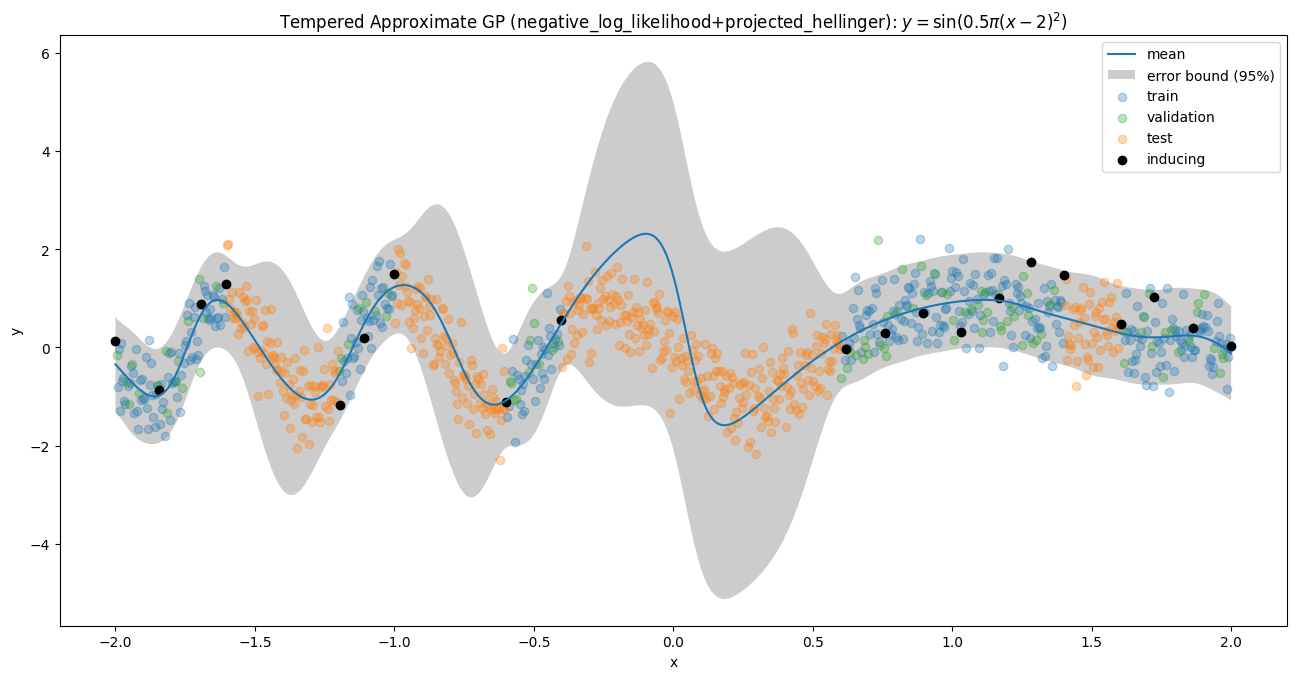
\includegraphics[width=\linewidth, trim={0 0 0 0.85cm},clip]{thesis_report/figures/toy_curves/curve8.png}
  \end{minipage}%
\begin{minipage}{.5\textwidth}
  \centering
  \textit{Curve 2}
  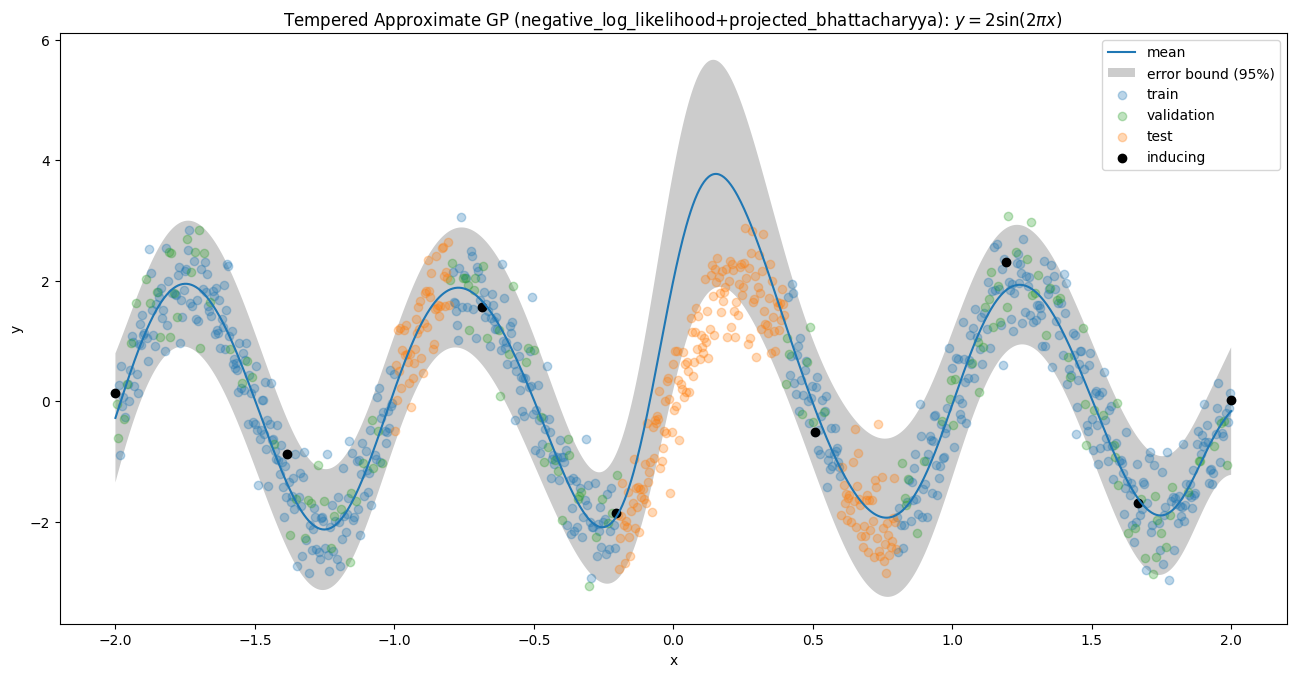
\includegraphics[width=\linewidth, trim={0 0 0 0.84cm},clip]{thesis_report/figures/toy_curves/curve1.png}
  \textit{Curve 4}
  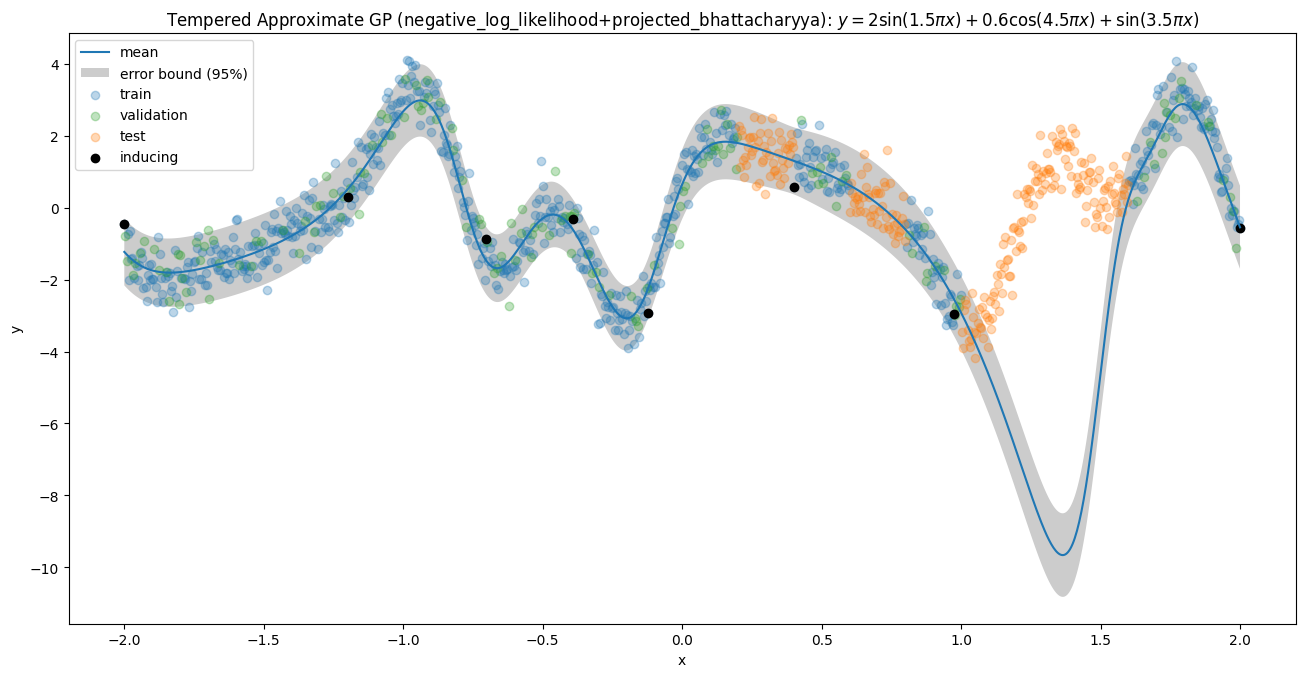
\includegraphics[width=\linewidth, trim={0 0 0 0.8cm},clip]{thesis_report/figures/toy_curves/curve3.png}
  \textit{Curve 6}
  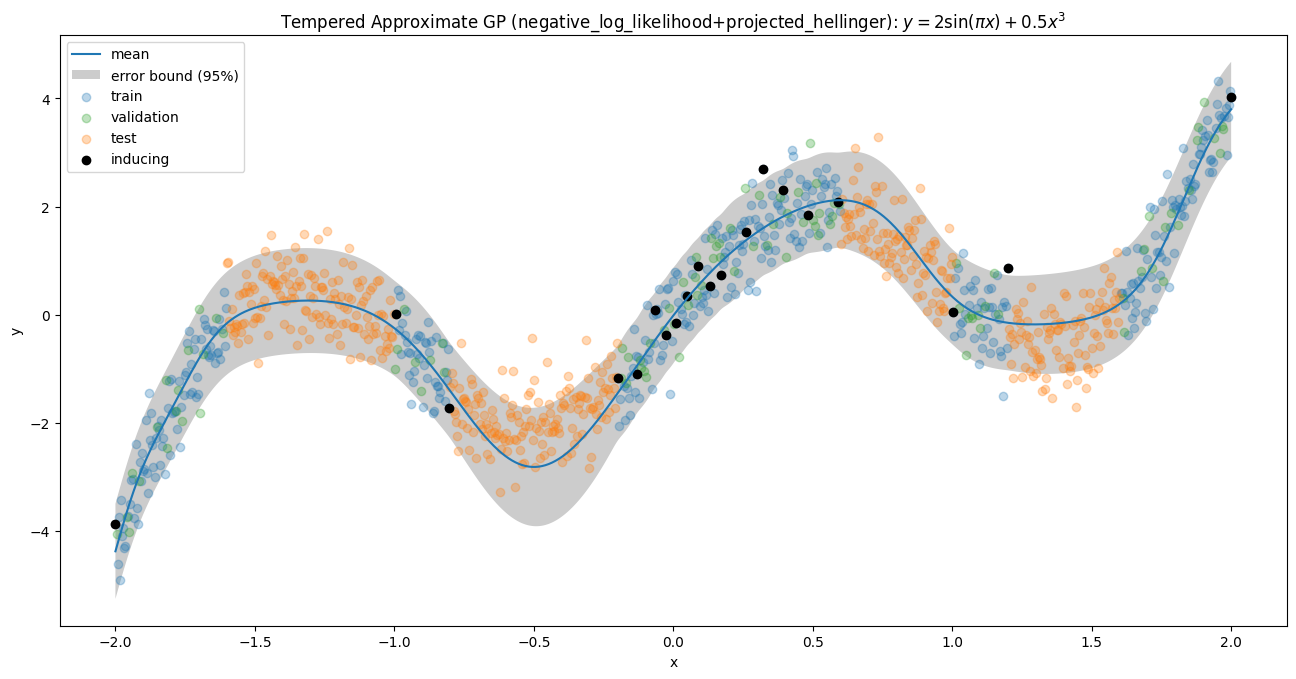
\includegraphics[width=\linewidth, trim={0 0 0 0.86cm},clip]{thesis_report/figures/toy_curves/curve5.png}
  \textit{Curve 8}
  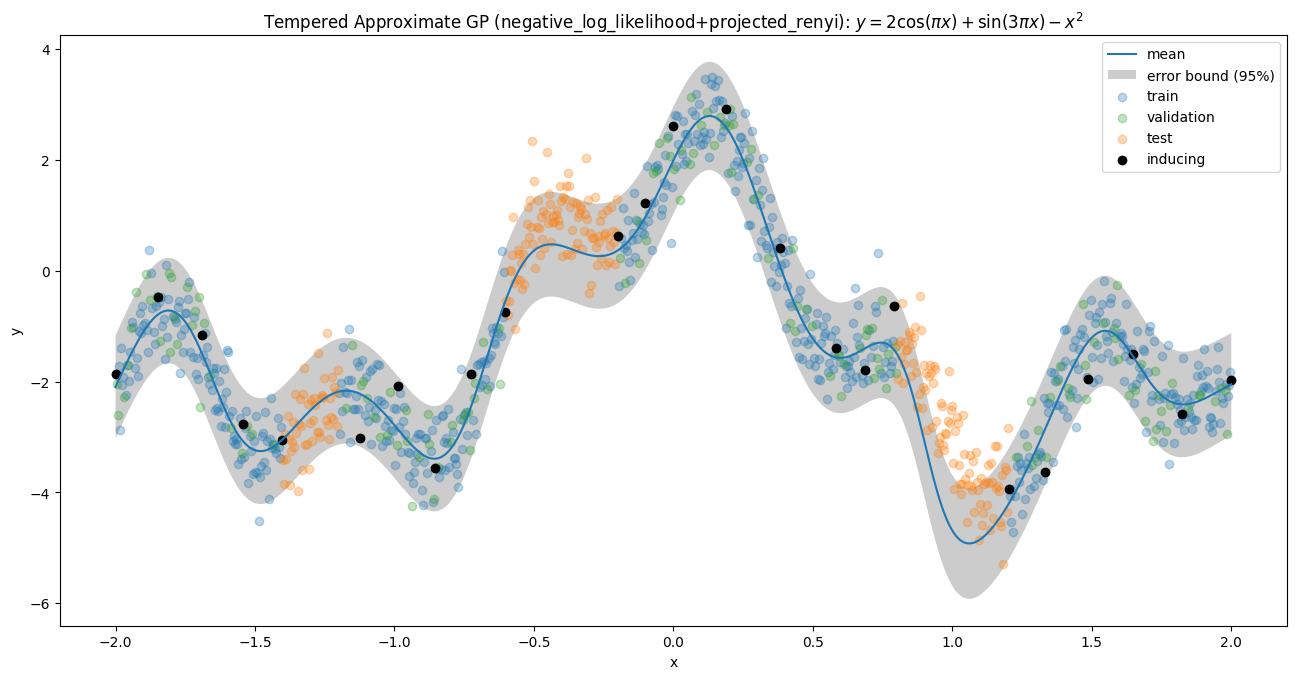
\includegraphics[width=\linewidth, trim={0 0 0 0.85cm},clip]{thesis_report/figures/toy_curves/curve7.png}
  \textit{Curve 10}
  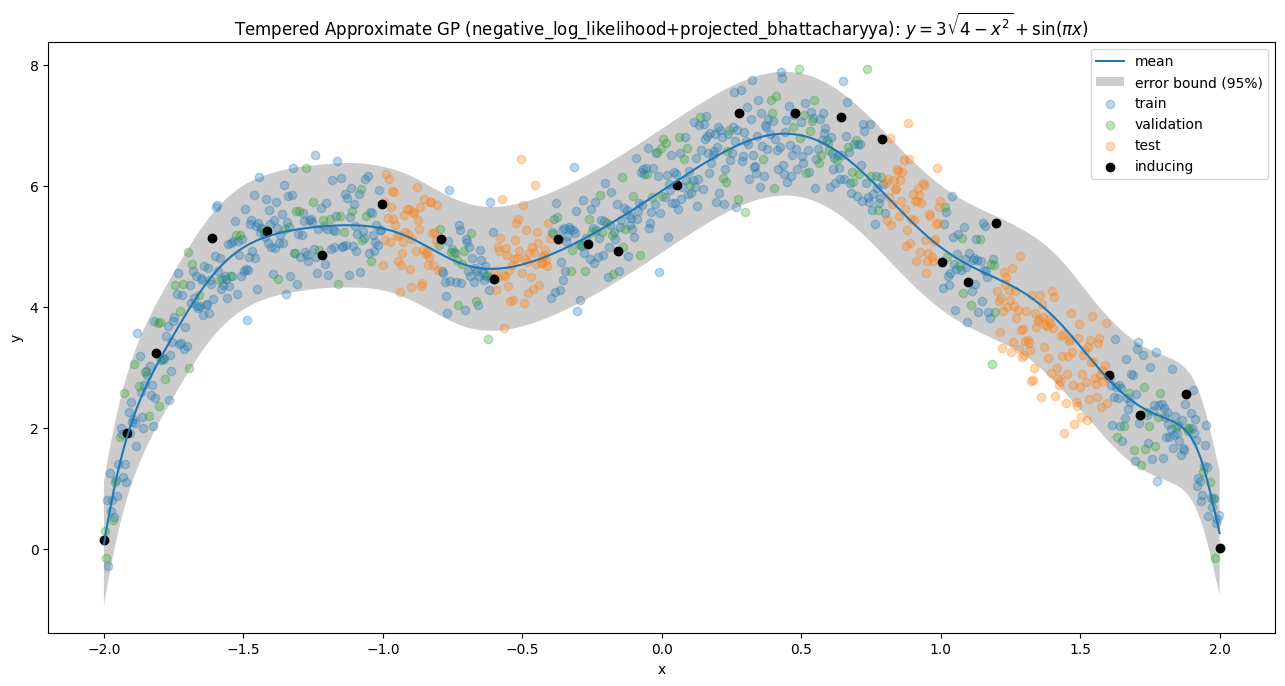
\includegraphics[width=\linewidth, trim={0 0 0 1.05cm},clip]{thesis_report/figures/toy_curves/curve9.png}
  \end{minipage}%
\caption{Best Performing Approximate GPs with respect to Validation Set NLL \textit{(black inducing points, blue training points, green validation points, and orange test points)}}
\label{figure:toy-curves-gps}
\end{figure}

The best performing approximate GPs are shown in Figure \ref{figure:toy-curves-gps}. Our framework is quite successful at learning the training data for all the curve examples.
With the exception of Curve 4, they also demonstrate reasonable behaviours in the OOD setting. 
Table \ref{table:toy-curve-configs} outlines the configurations for each best performing GP. 
Appendix \ref{appendix:configurations} contains further details for each setting.
Interestingly, in some cases it was actually better to use fewer inducing points with $M = \mathcal{O}(N^{1/3})$.
We also see that optimal settings can vary quite significantly.
This demonstrates the flexibility of GWI and pGVI to accommodate the specific variational space and learning objective that may be best suited for a given problem.
Please refer to the \code{experiments/toy\_curves/} directory to reproduce our results.

\begin{table}[h!]
\tiny
\centering
\begin{tabular}{lllllll}
\toprule
Problem &  $M = \mathcal{O}(N^{1/\alpha})$  &                      $k(x, x')$ &       $r(x, x')$ & $P$ Mode &   $\mathbb{D}[\wc, \wc]$ &  $\ell. r.$ \\
\midrule
 Curve 1  &                       $\alpha=2$ &                1-layer-tanh-fcnn-nngp &          diagonal-svgp &          prior &         proj-renyi &      1e-2 \\
 Curve 2  &                       $\alpha=3$ & 1-layer-tanh-fcnn-mapping-linear-base &       sparse-posterior &          prior & proj-bhattacharyya &      1e-4 \\
 Curve 3  &                       $\alpha=2$ &                                  ard &       sparse-posterior &      posterior &         proj-renyi &      1e-4 \\
 Curve 4  &                       $\alpha=3$ &                1-layer-tanh-fcnn-nngp &          diagonal-svgp &      posterior & proj-bhattacharyya &      1e-4 \\
 Curve 5  &                       $\alpha=2$ &                                  ard & fixed-sparse-posterior &          prior & proj-bhattacharyya &      1e-4 \\
 Curve 6  &                       $\alpha=2$ &                1-layer-tanh-fcnn-nngp &        kernelised-svgp &          prior &     proj-hellinger &      1e-2 \\
 Curve 7  &                       $\alpha=2$ &                                  ard &        kernelised-svgp &      posterior & proj-bhattacharyya &      1e-3 \\
 Curve 8  &                       $\alpha=2$ &                1-layer-tanh-fcnn-nngp &          diagonal-svgp &          prior &         proj-renyi &      1e-4 \\
 Curve 9  &                       $\alpha=2$ &                                  ard &        kernelised-svgp &      posterior &     proj-hellinger &      1e-4 \\
 Curve 10 &                       $\alpha=2$ &                                  ard &        kernelised-svgp &          prior & proj-bhattacharyya &      1e-2 \\
\bottomrule
\end{tabular}
\caption{Best Performing Settings with respect to Validation Set NLL}
\label{table:toy-curve-configs}
\end{table}


\newpage
\section{Future Work}\label{section:future-work}
This section discusses potential future extensions of our work. 
In particular, we will discuss applications to different problem domains that can push the limits of GWI and pGVI. 
This will hopefully provide additional feedback and understanding into the strengths and limitations of our approaches.
By leveraging our code base, most of these extensions will involve minimal implementation work.

% \paragraph{Fictitious Inducing Points} Algorithm \ref{alg:inducing-points-prior-gp} selects inducing points as a subset of existing training points within the training set.
% Limiting the selection space to the training data could be restrictive. 
% Learning `fictitious' inducing points that are not explicitly in the training data may help incorporate additional flexibility to the selection process.
% The \code{k-means++} algorithm proposed by \cite{arthur2007k} is another common approach to inducing point selection, identifying cluster centroids as potential inducing points.
% This moves away from having inducing point selection limited to a subset of the training data.
% Incorporating this approach into Algorithm \ref{alg:inducing-point-selection} and \ref{alg:inducing-points-prior-gp} may improve inducing point selection in certain data regimes.

\paragraph{UCI Regression Benchmarking} 
Many variational GP approaches such as \cite{wild2022generalized}, \cite{blundell2015weight}, \cite{gal2015dropout}, \cite{li2017dropout}, \cite{ma2021functional}, \cite{ma2019variational}, and \cite{sun2019functional} benchmark their approaches with standard UCI regression datasets. 
The next step in our work will be to benchmark the experimentation framework we proposed in Section \ref{section:experimentation-framework} with these datasets.
This will provide better understanding of GWI-GPs and pGVI-GPs within the context of the existing literature for function space VI.


\paragraph{Image Classification} 
A differentiating feature of GWI is the freedom to parameterise the variational GP with any mean and kernel. 
\cite{wild2022generalized} shows promising experimental results for GWI within the context of image classification by parameterising the variational mean with a CNN.
However, they use an ARD kernel to construct their svGP variational kernel.

We showed that the kernels in Section \ref{prior-kernels} have the potential to better quantify uncertainty in images by leveraging the more structured nature of the data.
A natural next step is to explore the performance of GWI-GPs and pGVI-GPs with these NNGP kernels and custom feature mapping kernels in combination with the new variational kernels proposed in Section \ref{variational-kernels}.
With the classification GP implementations in our code base, one could extend our current work to this use case with relative ease.

\paragraph{NLP Classification} GWI and pGVI introduces flexibility and computational performance previously unavailable to variational GP learning. 
This motivates us to explore the limits of these learning frameworks with larger data settings, such as problems in the Natural Language Processing (NLP) domain.
Candidate problems include sentiment analysis and named-entity recognition (NER), which would both be implementation extensions of an image classification model.

Attention networks are a fundamental building block for transformer models, the default architecture used by the NLP community at the moment. \cite{pmlr-v119-hron20a} proposes the existence of infinite-width attention networks.
These could be used to parameterise GPs within our VI frameworks.
Alternatively, the custom feature mapping kernel proposed in (\ref{custom-feature-map-kernel}) can accommodate any feature mapping for $h$, including pre-trained transformer embedding models. 
These would both be reasonable approaches for constructing variational GPs in the NLP domain.

\newpage
\section{Conclusions}\label{section:conclusions}
Generalised variational inference (GVI) proposed by \cite{knoblauch2022optimization} is an exciting development within the field of Bayesian inference.
An infinite dimensional realisation of GVI, Gaussian Wasserstein inference (GWI) from \cite{wild2022generalized}, establishes a new direction for function space variational inference, pivoting from previous approaches to the problem.
This has only started to demonstrate the potential of GVI, when applied to Gaussian processes (GPs). 


Through the modular nature of Algorithm \ref{alg:gwi-gp} and new kernel parameterisations, we further explored the flexibility of GWI.
With projected GVI (pGVI), we experimentally showed that weakening the assumption of a definite regulariser in GVI can still maintain a sensible loss objective for GP variational learning.
Compared to the cubic time complexity  of previous methods, projected regularisation is shown to be an attractive and practical linear time alternative. 
pGVI is an even more flexible learning framework and improves the accessibility of GPs for new problem domains that we hope to explore in the future.

Our proposed methods were developed in an experimentally-driven environment, primarily motivated to improve the computational and predictive performance of variational GPs. 
We hope that our contributions have inspired helpful insights into function space variational inference and will provide practical tools for future work with Gaussian processes.


\newpage
\bibliography{references}


\newpage
\appendix
\counterwithin{figure}{subsection}
\counterwithin{table}{subsection}
\section{Appendix}

\subsection{Positive Semi-Definite Kernels} \label{appendix:positive-definite-kernel}
Given a kernel function $k: \mathcal{X} \times \mathcal{X} \rightarrow \mathbb{R}$ defined as an inner product of features in some feature space $\mathcal{H}$ such that
\begin{align}
    k(x, x') = \langle \phi(x), \phi(x') \rangle_{\mathcal{H}},
\end{align}
where $\phi: \mathcal{X} \rightarrow \mathcal{H}$, a gram matrix $\mathbf{K} \in \mathbb{R}^{N\times N}$ defined element-wise as
\begin{align}
    \left[\mathbf{K}\right]_{n, n'} = k(x_n, x_{n'})
\end{align}
for any $N$ points $\mathbf{X} = \left\{x_n\right\}_{n=1}^N$ with $x_n \in \mathcal{X}$, and any vector $\mathbf{v} \in \mathbb{R}^N$ then
\begin{align}
    \mathbf{v}^T \mathbf{K} \mathbf{v} &= \sum_{n=1}^N\sum_{n'=1}^N v_n v_{n'}  \left\langle \phi(x_n), \phi(x_{n'}) \right\rangle_{\mathcal{H}} \\
    &= \left\langle\sum_{n=1}^N v_n \phi(x_n), \sum_{n'=1}^N  v_{n'}\phi(x_{n'}) \right\rangle_{\mathcal{H}} \\
    &= \left\| \sum_{n=1}^N v_n \phi(x_n) \right\|^2 \geq 0
\end{align}
showing that $\mathbf{K}$ is a positive semi-definite matrix.

\newpage
\subsection{Symmetric Matrix Eigenvalues}\label{appendix:eigenvalue-symmetric-matrix}
For square symmetric matrices $\mathbf{A}, \mathbf{B} \in \mathbb{R}^{N \times N}$, $\sqrt{\mathbf{A}}\mathbf{B}\sqrt{\mathbf{A}}$ is also a symmetric matrix where $\sqrt{\mathbf{A}}$ is the square root such that $\mathbf{A} = \sqrt{\mathbf{A}}^T \sqrt{\mathbf{A}}$. Moreover, it can be shown that
\begin{align}
    \lambda_{n} \left(\mathbf{A} \mathbf{B}\right) = \lambda_{n} \left(\sqrt{\mathbf{A}}\mathbf{B}\sqrt{\mathbf{A}}\right)
\end{align}
for all $n=1,\dots,N$, where $\lambda_{n}(\cdot)$ computes the $n^{th}$ eigenvalue.

\newpage
\subsection{Example Experiment Configurations}\label{appendix:configuration-yamls}
\begin{figure}[!h]
\begin{lstlisting}[style=yaml]
data_name: 604913dc3af2417fb1d5a21ea26e4afd
empirical_risk_break_condition: -10
empirical_risk_schema: negative_log_likelihood
inducing_points:
  inducing_points_factor: 1.0
  inducing_points_power: 3
  inducing_points_selector_schema: conditional_variance
kernel:
  kernel_kwargs:
    input_shape:
    - 1
    layers:
      layer_1:
        layer_kwargs:
          features: 10
        layer_schema: dense
      layer_2:
        layer_kwargs: null
        layer_schema: tanh
  kernel_parameters: null
  kernel_schema: nngp
number_of_iterations: 5
save_checkpoint_frequency: 1000
trainer_settings:
  batch_drop_last: false
  batch_shuffle: true
  batch_size: 1000
  learning_rate: 0.0001
  number_of_epochs: 10000
  optimiser_schema: adabelief
  seed: 0
\end{lstlisting}
\caption{Regulariser GP Example Configuration YAML}
\end{figure}

\newpage
\begin{figure}[!h]
\begin{lstlisting}[style=yaml]
empirical_risk_schema: negative_log_likelihood
kernel:
  kernel_kwargs:
    diagonal_regularisation: 1.0e-10
    is_diagonal_regularisation_absolute_scale: false
  kernel_parameters: null
  kernel_schema: sparse_posterior
mean:
  mean_kwargs:
    nn_function_kwargs:
      input_shape:
      - 1
      layers:
        layer_1:
          layer_kwargs:
            features: 10
          layer_schema: dense
        layer_2:
          layer_kwargs: null
          layer_schema: tanh
        layer_3:
          layer_kwargs:
            features: 1
          layer_schema: dense
      seed: 0
    number_output_dimensions: 1
  mean_parameters: null
  mean_schema: custom
reference_name: 7b386a3faf1f4b79ac6ff6604b6bc932
regularisation:
  regularisation_kwargs:
    mode: posterior
    alpha: 0.5
  regularisation_schema: projected_renyi
save_checkpoint_frequency: 1000
trainer_settings:
  batch_drop_last: false
  batch_shuffle: true
  batch_size: 1000
  learning_rate: 0.001
  number_of_epochs: 50000
  optimiser_schema: adabelief
  seed: 0
\end{lstlisting}
\caption{Approximate GP Example Configuration YAML}
\end{figure}
\newpage 
\subsection{Regression Curve Experiment Settings}\label{appendix:configurations}
The following tables outline the options for each setting in Table \ref{table:toy-curve-configs}. 
Taking all combinations of these settings generates 1260 unique experiments.

\begin{table}[h!]
\tiny
\centering
\begin{tabular}{r}
\toprule
 $M = \mathcal{O}\left(N^{1/\alpha}\right)$ \\
\midrule
                                 $\alpha=2$ \\
                                 $\alpha=3$ \\
\bottomrule
\end{tabular}
\caption{Number of Inducing Points \textit{($\alpha$ is the root factor)}}
\end{table}

\begin{table}[h!]
\tiny
\centering
\begin{tabular}{ll}
\toprule
             $k(x, x')$ & Description\\
\midrule
1-layer-tanh-fcnn-mapping-linear & Feature Mapping Kernel: single-layer FCNN \& tanh activations with linear base kernel\\
          1-layer-tanh-fcnn-nngp &  NNGP Kernel: single-layer FCNN \& tanh activations\\
                            ard & ARD Kernel\\
\bottomrule
\end{tabular}
\caption{Regulariser GP Kernel}
\end{table}

\begin{table}[h!]
\tiny
\centering
\begin{tabular}{l}
\toprule
    $r(x, x')$ \\
\midrule
         cholesky-svgp \\
         diagonal-svgp \\
fixed-sparse-posterior \\
       kernelised-svgp \\
      sparse-posterior \\
\bottomrule
\end{tabular}
\caption{Approximate GP Kernel}
\end{table}

\begin{table}[h!]
\tiny
\centering
\begin{tabular}{l}
\toprule
$P$ Mode \\
\midrule
                      posterior \\
                          prior \\
\bottomrule
\end{tabular}
\caption{Regulariser GP Mode}
\end{table}

\begin{table}[h!]
\tiny
\centering
\begin{tabular}{l}
\toprule
  $\mathbb{D}[\wc, \wc]$ \\
\midrule
            proj-bhattacharyya \\
                proj-hellinger \\
                       proj-kl \\
                    proj-renyi \\
proj-squared-difference \\
     proj-wasserstein \\
       wasserstein-partial \\
\bottomrule
\end{tabular}
\caption{GVI Regularisation \textit{(`partial' indicates dropping the eigendecomposition term)}}
\end{table}

\begin{table}[h!]
\tiny
\centering
\begin{tabular}{r}
\toprule
 $\ell. r.$ \\
\midrule
                    1e-2 \\
                    1e-3 \\
                    1e-4 \\
\bottomrule
\end{tabular}
\caption{GVI Learning Rate}
\end{table}

\end{document}x